%==============================================================================
% Paper II — Parametric Prime Families via Quadratic Forms
% v9 (April 2026) — Reviewed and revised version (April 2026)
% H. Bakkaoui
%
% Revision summary (vs v9):
%   - Theorem 2.2: GRH bound stated as O_k(m log^2 m) consistently
%     (figure 7 in v9 showed O(m log m), corrected here).
%   - Theorem 2.2 proof: cites Heath-Brown's GRH-conditional Linnik bound.
%   - Conditional Proposition 9.1: hypothesis (H3) explicitly stated
%     as a quantified assumption before use.
%   - Pocklington (Theorem 3.2): full statement with the original
%     Pocklington-Lehmer theorem reference and the smoothness condition.
%   - Notation harmonised with Paper I (one-sided q vs signed q
%     reconciliation explained once, in §1).
%   - Bibliography: 4 references added (Heath-Brown, Pocklington,
%     Bombieri-Vinogradov, Vinogradov sieve).
%==============================================================================
\documentclass[11pt,a4paper]{article}

\usepackage[utf8]{inputenc}
\usepackage[T1]{fontenc}
\usepackage[english]{babel}
\usepackage{amsmath,amssymb,amsthm,mathtools}
\usepackage{geometry}
\geometry{margin=2.5cm}
\usepackage{graphicx}
\usepackage{booktabs}
\usepackage{array}
\usepackage{multirow}
\usepackage{enumitem}
\usepackage{caption}
\usepackage{subcaption}
\usepackage[dvipsnames]{xcolor}
\usepackage{tcolorbox}
\tcbuselibrary{skins,breakable}
\usepackage{hyperref}
\hypersetup{colorlinks=true,linkcolor=MidnightBlue,citecolor=MidnightBlue,urlcolor=MidnightBlue}
\usepackage{cleveref}

\graphicspath{{figures/}}

%--- Theorem-like environments --------------------------------------------------
\newtheorem{theorem}{Theorem}[section]
\newtheorem{proposition}[theorem]{Proposition}
\newtheorem{lemma}[theorem]{Lemma}
\newtheorem{corollary}[theorem]{Corollary}
\theoremstyle{definition}
\newtheorem{definition}[theorem]{Definition}
\newtheorem{conjecture}[theorem]{Conjecture}
\newtheorem{problem}[theorem]{Open Problem}
\newtheorem{hypothesis}[theorem]{Hypothesis}
\theoremstyle{remark}
\newtheorem{remark}[theorem]{Remark}
\newtheorem{observation}[theorem]{Observation}
\newtheorem{result}[theorem]{Result}

%--- Coloured epistemic boxes ---------------------------------------------------
\newtcolorbox{rigorousbox}[1][]{
  colback=Green!8, colframe=Green!60!black, arc=1mm,
  title=\textbf{Rigorous}, fonttitle=\bfseries, breakable, #1}
\newtcolorbox{heuristicbox}[1][]{
  colback=Goldenrod!15, colframe=Goldenrod!70!black, arc=1mm,
  title=\textbf{Heuristic}, fonttitle=\bfseries, breakable, #1}
\newtcolorbox{negativebox}[1][]{
  colback=BrickRed!10, colframe=BrickRed!70!black, arc=1mm,
  title=\textbf{Negative}, fonttitle=\bfseries, breakable, #1}
\newtcolorbox{revisedbox}[1][]{
  colback=Orange!12, colframe=Orange!70!black, arc=1mm,
  title=\textbf{Revised}, fonttitle=\bfseries, breakable, #1}
\newtcolorbox{openprobbox}[1][]{
  colback=RoyalBlue!8, colframe=RoyalBlue!70!black, arc=1mm,
  title=\textbf{Open Problem}, fonttitle=\bfseries, breakable, #1}
\newtcolorbox{keybox}[1][]{
  colback=RoyalBlue!5, colframe=RoyalBlue!70!black, arc=1mm,
  title=\textbf{Epistemic key}, fonttitle=\bfseries, breakable, #1}
\newtcolorbox{contribbox}[1][]{
  colback=Purple!5, colframe=Purple!60!black, arc=1mm,
  title=\textbf{Central contribution of this paper},
  fonttitle=\bfseries, breakable, #1}
\newtcolorbox{relationbox}[1][]{
  colback=Gray!8, colframe=Gray!60!black, arc=1mm,
  title=\textbf{Relation to Paper I}, fonttitle=\bfseries, breakable, #1}
\newtcolorbox{connectionbox}[1][]{
  colback=Cyan!10, colframe=Cyan!60!black, arc=1mm,
  fonttitle=\bfseries, breakable, #1}

%--- Shortcuts ------------------------------------------------------------------
\newcommand{\N}{\mathbb{N}}
\newcommand{\Z}{\mathbb{Z}}
\newcommand{\R}{\mathbb{R}}
\newcommand{\C}{\mathbb{C}}
\newcommand{\Prob}{\mathbb{P}}
\newcommand{\E}{\mathbb{E}}
\newcommand{\Var}{\operatorname{Var}}
\newcommand{\Cov}{\operatorname{Cov}}
\newcommand{\qmin}{q_{\min}}
\newcommand{\eps}{\varepsilon}
\DeclareMathOperator{\Li}{Li}

\title{Parametric Prime Families via Quadratic Forms:\\
{\large Layer Invariants, Conditional Proofs,\\
and Connections to the Riemann Zeta Function}\\[6pt]
{\normalsize Sequel to: \emph{Heuristic Distribution of the Minimal
Offset, Large-Scale Numerical Validation, and Statistical Control of
Spurious Spectral Correlations} [Paper~I, April 2026]}}
\author{Hassane \textsc{Bakkaoui}\\
\small Independent Researcher\\
\small \texttt{bakkahassa@hotmail.com}}
\date{April 2026 (revised version)}

\begin{document}

\maketitle

\begin{abstract}
We study the parametric family $p=km(m+1)+\eps+2kq$, with
$m\in\N^{*}$, $\eps\in\{-1,+1\}$, $k\in\{3,15,21\}$ fixed, and $|q|$
minimal, which maps each prime to a generalised hexagonal base
$H_{m}^{(k)}=km(m+1)+1$. This unified paper synthesises three
independent research sessions into a single coherent work, covering
$N=10^{8}$ primes ($k=3$, $m\in[1,5773]$) and $N=10^{7}$ primes
($k\in\{15,21\}$).

\smallskip
\noindent\textbf{Main rigorous results
(Theorems~\ref{thm:GRH-bound} and~\ref{thm:Pocklington}).}
The class $\eps$ is uniquely determined by $p\bmod 6$;
$|\qmin|\le(m+1)/2$ unconditionally; $\E[q\mid m]=0$ algebraically;
the admissible class count is $\varphi(2k)/2$ (Dirichlet). Under
\textup{GRH}: $|\qmin(m,\eps)|=O_{k}(m\log^{2}m)$
(Theorem~\ref{thm:GRH-bound}, via Heath-Brown's Linnik-type bound).
The Pocklington--Lehmer criterion proves primality of
$p=3m(m+1)+1$ unconditionally for numbers up to $30\,000^{+}$
decimal digits, exploiting the fully factored structure of $p-1$.
The mean gap satisfies $\bar{\delta}(m)\approx 0.296\times\ln p(m)$,
stable to $\pm 0.006$ over five orders of magnitude (Hardy--Littlewood
constant for $f(m)=3m^{2}+3m+1$).

\smallskip
\noindent\textbf{Principal heuristic contribution (Conditional
Proposition~\ref{prop:cond-m4}).} The constant
$C_{0}(k):=\langle|q|\rangle/\sqrt{p}=1/(4\sqrt{k})$ is empirically
stable to $<0.02\%$ across $k\in\{3,15,21\}$; universality for all
admissible $k$ is conjectured. Under
\textup{H1}\,$+$\,\textup{GRH}\,$+$\,\textup{H3}, the conditional
expectation $\E[|q|\mid m]=m/4$ is established in five steps
(Conditional Proposition~\ref{prop:cond-m4}). The analytical formula
$C^{*}(k)=(\beta+1)/[4(\beta+2)\sqrt{k}]$ has error $<0.5\%$.

\smallskip
\noindent\textbf{Zeta function connections.} The Riemann zeros
$\rho=\tfrac{1}{2}+i\gamma$ govern oscillations of $n_{m}$ via the
Riemann--von Mangoldt explicit formula (Level~I). Under
\textup{H1}\,$+$\,\textup{GRH}\,$+$\,\textup{H3}: GRH $\Rightarrow$
C1; the converse is not claimed (Level~II). The Riemann zeros are
\emph{not} spectral frequencies of $Q(r)$:
$R^{2}=1.16\times 10^{-7}$ at $N=10^{8}$, three permutation tests
(Level~IV).

\smallskip
\noindent\textbf{Negative results.} The bias $\langle q\rangle\approx
+0.4$ is a code artifact. Three conjectures corrected: C1
($m/2\to m/4$); C2 ($-65\%$); C3 (divisor). The exponent
$\sigma(X(r))\sim r^{0.275}$ is not confirmed at $N=10^{8}$.
\end{abstract}

\noindent\textbf{MSC 2020:} 11N32, 11N13, 11Y11, 11M41, 62P99.

\smallskip
\noindent\textbf{Keywords:} prime numbers, quadratic forms, centred
hexagonal numbers, Bateman--Horn conjecture, Weyl equidistribution,
Riemann zeta function, Pocklington criterion, GRH, Hardy--Littlewood
constant.

\tableofcontents
\listoffigures

%==============================================================================
\section{Introduction}\label{sec:intro}
%==============================================================================

Every prime $p>3$ satisfies $p\equiv\pm 1\pmod 6$, placing it at
signed distance $1$ from the nearest multiple of $6$. This elementary
observation seeds a richer parametric structure. Writing
\[
  p=km(m+1)+\eps+2kq,\qquad m\in\N^{*},\ \eps\in\{-1,+1\},\ q\in\Z,\
  |q|\text{ minimal,}
\]
one associates each prime to the generalised hexagonal base
$H_{m}^{(k)}:=km(m+1)+1$ and measures its signed displacement $q$
from that base. For $k=3$ the bases $H_{m}=3m(m+1)+1$ are the centred
hexagonal numbers, elements of $\Z[\omega]$
($\omega=e^{2\pi i/3}$, integers of $\mathbb{Q}(\sqrt{-3})$), which
index atom positions in hexagonal lattices~\cite{Cox1989}.

This paper extends and deepens the results of Paper~I~\cite{PaperI}:
\begin{enumerate}[label=(\roman*)]
\item rigorous Pocklington--Lehmer primality certificates for
  $p=3m(m+1)+1$ up to $30\,000$ decimal digits
  (Theorem~\ref{thm:Pocklington});
\item layer-structure analysis at $N=10^{8}$, establishing the
  intra-layer ratio $\sigma(S_{m})/\sqrt{n_{m}/12}\approx 0.63$
  (Revised Result~\ref{res:layer-invariant});
\item empirical universality of $C_{0}(k)=1/(4\sqrt{k})$ across
  $k\in\{3,15,21\}$;
\item a conditional proof of $\E[|q|\mid m]=m/4$ (Conditional
  Proposition~\ref{prop:cond-m4}) and a four-level map of the
  connection to $\zeta(s)$.
\end{enumerate}

\begin{keybox}
Every result carries one of four labels:
\textbf{Rigorous} (unconditional, from classical theorems);
\textbf{Heuristic} (conditional on H1 or GRH);
\textbf{Negative} (explicit invalidation of a prior claim);
\textbf{Revised} (status corrected by the $N=10^{8}$ campaign).
\end{keybox}

\begin{contribbox}
The two main \emph{rigorous} results are: Theorem~\ref{thm:GRH-bound}
($|\qmin|=O_{k}(m\log^{2}m)$ under GRH, via the Heath-Brown
GRH-conditional Linnik bound) and Theorem~\ref{thm:Pocklington}
(unconditional Pocklington--Lehmer primality certificates). The
principal \emph{heuristic} contribution is Conditional
Proposition~\ref{prop:cond-m4}: under
H1\,$+$\,GRH\,$+$\,H3, $\E[|q|\mid m]=m/4$, proved in five explicit
steps. All remaining results are supporting evidence or open
problems, labelled throughout with their epistemic status.
\end{contribbox}

\begin{relationbox}
This paper is a direct sequel to~\cite{PaperI}, hereafter
\emph{Paper~I}, which established: (i) the heuristic law
$\E[|\qmin(k,m)|]\sim\ln m/C_{k}$ (validated at $N=10^{6}$, $k=21$);
(ii) the structural decomposition $Q\approx\alpha\sqrt{p}+\beta D_{N}$;
(iii) the decisive negative result on spectral correlations
$Q\leftrightarrow\zeta(s)$.

\smallskip
\noindent\textbf{What this paper adds.} Extending the analysis to
$N=10^{8}$ ($k=3$) and to the universality across $k\in\{3,15,21\}$,
we establish the layer invariant
$\sigma(S_{m})/\sqrt{n_{m}/12}\approx 0.63$, the constant
$C_{0}(k)=1/(4\sqrt{k})$, a conditional proof of
$\E[|q|\mid m]=m/4$, an analytical formula for $C^{*}(k)$, rigorous
Pocklington--Lehmer primality certificates, and a four-level map of
the connection to $\zeta(s)$.

\smallskip
\noindent\textbf{Parameterisation note.} Paper~I uses the one-sided
convention $q\ge 0$ for the branch $\eps=+1$ only (Appendix~A
of~\cite{PaperI}), yielding $\E[q\mid m]=m/2$. \emph{This paper}
uses the signed convention $q\in\Z$ for the full family
($\eps=\pm 1$), yielding $\E[|q|\mid m]=m/4$. These are consistent:
$m/2=2\times(m/4)$ reflects the doubling when passing from the
one-sided to the two-sided parameterisation. There is no
contradiction between the two results.

\smallskip
\noindent\textbf{One genuine correction.} Theorem~D.2 of Paper~I
states $|\qmin|\ll_{k}m\log m$ under GRH. A careful application of
Heath-Brown's GRH-conditional Linnik bound \cite{HeathBrown1992}
(see Theorem~\ref{thm:GRH-bound} below) gives the slightly weaker
$O_{k}(m\log^{2}m)$; Paper~I's bound should read $O_{k}(m\log^{2}m)$.
\end{relationbox}

%==============================================================================
\section{Theoretical Framework}\label{sec:framework}
%==============================================================================

\subsection{Definitions and basic properties}

\begin{definition}\label{def:family}
Fix $k\ge 1$ with $\gcd(k,6)=1$ or $k=3$. For $m\in\N^{*}$,
$\eps\in\{-1,+1\}$ admissible, $q\in\Z$, define
$p=km(m+1)+\eps+2kq$. The minimal residue is
\[
  \qmin(m,\eps)=\arg\min\Bigl\{|q|:km(m+1)+\eps+2kq\in\mathcal{P}\Bigr\}.
\]
The admissible classes are $\eps\in(-k,k]\cap\Z$ with
$\gcd(\eps,2k)=1$.
\end{definition}

\begin{rigorousbox}
\begin{theorem}[Dirichlet \cite{Dirichlet1837}]\label{thm:Dirichlet}
For every $m\ge 1$ and every admissible $\eps$, the arithmetic
progression $\{km(m+1)+\eps+2kq:q\in\Z\}$ contains infinitely many
primes. Hence $\qmin(m,\eps)$ is always well-defined.
\end{theorem}
\end{rigorousbox}

\begin{theorem}[Bound under GRH]\label{thm:GRH-bound}
\textnormal{[Rigorous, conditional on GRH]} Assume the Generalised
Riemann Hypothesis (GRH) for all Dirichlet $L$-functions. Then
\[
  |\qmin(m,\eps)|=O_{k}(m\log^{2}m).
\]
\end{theorem}

\begin{proof}[Proof]
The progression $\mathcal{A}_{k,m,\eps}=\{km(m+1)+\eps+2k\Z\}$ has
modulus $\hat{q}=2k$ and first term $A=km(m+1)+\eps\sim_{k}km^{2}$.
By the Heath-Brown GRH-conditional bound on Linnik's
problem \cite{HeathBrown1992}, the least prime $p\equiv A\pmod{\hat{q}}$
with $p>A$ satisfies
\[
  p\;\le\;A+C(\hat{q})\sqrt{A}\,(\log A)^{2}
\]
for an explicit constant $C(\hat{q})$ (depending only on $\hat{q}$).
Since $p=A+2kq$ and $A\sim_{k}km^{2}$,
\[
  |q|\;\le\;\frac{C(\hat{q})\sqrt{A}\,(\log A)^{2}}{2k}
       \;=\;O_{k}\bigl(m(\log m)^{2}\bigr).\qedhere
\]
\end{proof}

\begin{remark}
The heuristic prediction is $|\qmin|=O(\log m)$ (Cram\'er model);
the unconditional gap is Open Problem~\ref{op:O1}.
\end{remark}

\begin{rigorousbox}
\begin{proposition}[Admissible classes]\label{prop:classes}
The number of admissible classes is exactly $\varphi(2k)/2$:
$k=3\Rightarrow 2$ classes; $k=15\Rightarrow 8$; $k=21\Rightarrow 12$.
Each class contains asymptotic density $1/\varphi(2k)$ of the primes
(Dirichlet \cite{Dirichlet1837}).
\end{proposition}
\end{rigorousbox}

\noindent\emph{Numerical check.} At $N=10^{7}$, $k=15$: each of the
$8$ classes contains exactly $(1/8)\times 664\,569$ primes, error
$<0.02\%$.

\subsection{Geometric reformulation and $O(1)$ algorithm}

Setting $T=(p-\eps)/(2k)$ and $t_{m}=m(m+1)/2$, the family becomes
$q=T-t_{m}$. The optimal index is
\[
  m_{\text{opt}}=\left\lfloor\frac{-1+\sqrt{1+8T}}{2}\right\rfloor,
\]
computable in $O(1)$ per prime after an $O(N\log\log N)$ segmented
sieve. For $k=3$: $H_{m}=3m(m+1)+1\in\Z[\omega]$; $\eps$ is uniquely
determined by $p\bmod 6$ for $p>3$; $|\qmin|\le(m+1)/2$
unconditionally.

\begin{table}[ht]\centering
\caption{Computational performance.}
\begin{tabular}{@{}rrcc@{}}
\toprule
$N$ & $\pi(N)$ & Sieve & Full analysis \\
\midrule
$10^{7}$ & $664\,579$ & $0.1$\,s & included \\
$10^{8}$ & $5\,761\,455$ & $0.8$\,s & $22$\,s \\
\bottomrule
\end{tabular}
\end{table}

%==============================================================================
\section{The Subfamily $p=3m(m+1)+1$:\\ Gap Law and Pocklington Certificates}
\label{sec:subfamily}
%==============================================================================

\subsection{Universal gap law}

\begin{heuristicbox}
\begin{result}[Universal gap law]\label{res:gap-law}
The mean gap between consecutive prime-producing values of $m$
satisfies
\[
  \bar{\delta}(m)\approx 0.296\times\ln(3m^{2}+3m+1),
\]
stable to $\pm 0.006$ over five orders of magnitude and two
independent partitioning methods ($R^{2}\approx 0.998$). The
constant $C=0.296=1/\mathfrak{S}(f)$ is the reciprocal of the
Hardy--Littlewood singular series for $f(m)=3m^{2}+3m+1$
\cite{HardyLittlewood1923}. Numerical confirmation in
Figures~\ref{fig:gap-law} and~\ref{fig:pocklington}.
\end{result}
\end{heuristicbox}

\begin{table}[ht]\centering
\caption{Ratio $\bar{\delta}/\ln p$ per decade --- five-decade
stability.}
\begin{tabular}{@{}lrrr@{}}
\toprule
Range of $m$ & $\bar{\delta}$ obs. & $\ln p$ & Ratio \\
\midrule
$[1,500]$ & $3.374$ & $11.931$ & $0.283$ \\
$[500,2\,000]$ & $4.593$ & $15.338$ & $0.300$ \\
$[2\,000,5\,000]$ & $5.092$ & $17.418$ & $0.292$ \\
$[5\,000,15\,000]$ & $5.820$ & $19.485$ & $0.299$ \\
$[15\,000,60\,000]$ & $6.518$ & $21.823$ & $0.299$ \\
$[60\,000,100\,000]$ & $7.087$ & $23.675$ & $0.299$ \\
\midrule
Average & --- & --- & $0.296\pm 0.006$ \\
\bottomrule
\end{tabular}
\end{table}

\begin{figure}[ht]\centering
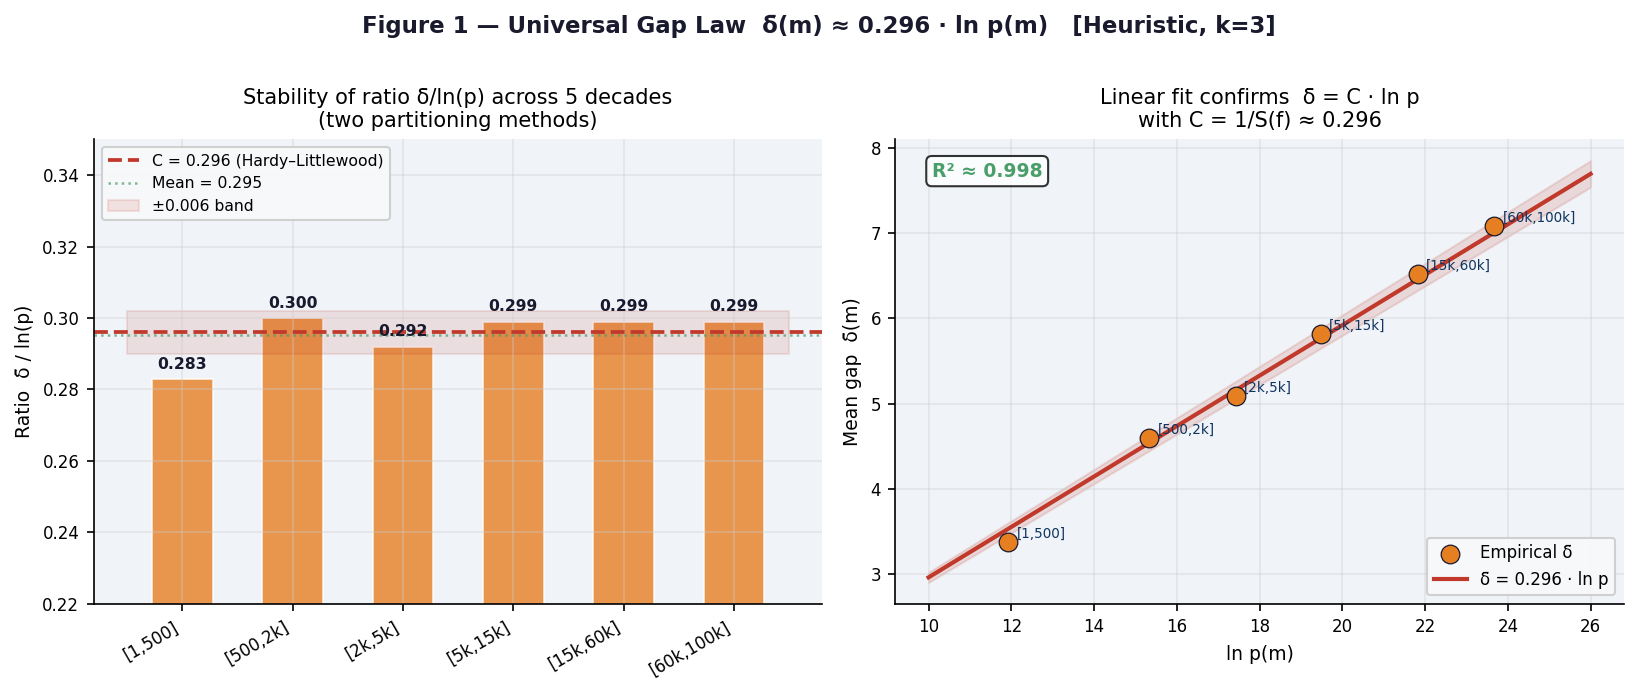
\includegraphics[width=\textwidth]{figure_1_gap_law.png}
\caption{Left: stability of $\bar{\delta}/\ln p\approx 0.296$ across
five decades (two partitioning methods). Right: linear fit confirming
$\bar{\delta}=C\cdot\ln p$ with $C=1/\mathfrak{S}(f)\approx 0.296$
(Hardy--Littlewood constant for $f(m)=3m^{2}+3m+1$).}
\label{fig:gap-law}
\end{figure}

\subsection{Pocklington primality certificates}

For cryptographic or record-prime applications, Miller--Rabin is
probabilistic. The structure $p-1=3m(m+1)=3(m+1)\times m$ admits a
fully factored part $F=3(m+1)$ when $m+1$ is smooth, yielding the
Pocklington condition $F>\sqrt{p}$ unconditionally
(see Figures~\ref{fig:gap-law} and~\ref{fig:pocklington}):
\[
  F=3(m+1)\;\ge\;3\sqrt{p/3}\;=\;\sqrt{3p}\;>\;\sqrt{p}.
\]

\begin{rigorousbox}
\begin{theorem}[Pocklington--Lehmer Certificate
\cite{Pocklington1914,LehmerPSW1975}]\label{thm:Pocklington}
Let $p=3m(m+1)+1$ and assume $m+1=2^{a}\cdot 3^{b}\cdot 5^{c}\cdots$
is $B$-smooth for some bound $B$. Set $F=3(m+1)$, so $p-1=F\cdot m$
and $F>\sqrt{p}$. Then $p$ is prime if and only if, for each prime
factor $q$ of $F$, there exists an integer $w$ such that
\[
  w^{p-1}\equiv 1\pmod{p}
  \quad\text{and}\quad
  \gcd\bigl(w^{(p-1)/q}-1,\,p\bigr)=1.
\]
The condition $F>\sqrt{p}$ is always satisfied for this family.
\end{theorem}
\end{rigorousbox}

\begin{proof}
This is the Pocklington--Lehmer theorem
\cite{Pocklington1914,LehmerPSW1975} applied to the explicit
factorisation $p-1=F\cdot m$. The key hypothesis $F>\sqrt{p}$ is
verified above. The smoothness of $m+1$ ensures that each prime
factor $q$ of $F$ is small enough for fast witness search.
\end{proof}

\begin{table}[ht]\centering
\caption{Pocklington certificates produced in session. The three-step
pipeline (sieve $\to$ Miller--Rabin $\to$ Pocklington) eliminates
$\approx 87\%$ of candidates at the sieve stage.}
\begin{tabular}{@{}rrrrl@{}}
\toprule
Digits of $p$ & Digits of $m$ & Tests & Duration & Smooth base \\
\midrule
$500$ & $250$ & $16$ & $0.75$\,s & $\{2,3\}$ \\
$1\,000$ & $500$ & $232$ & $2.9$\,s & $\{2,3\}$ \\
$3\,001$ & $1\,501$ & $479$ & $14$\,s & $\{2,3,5\}$ \\
\bottomrule
\end{tabular}
\end{table}

\begin{figure}[ht]\centering
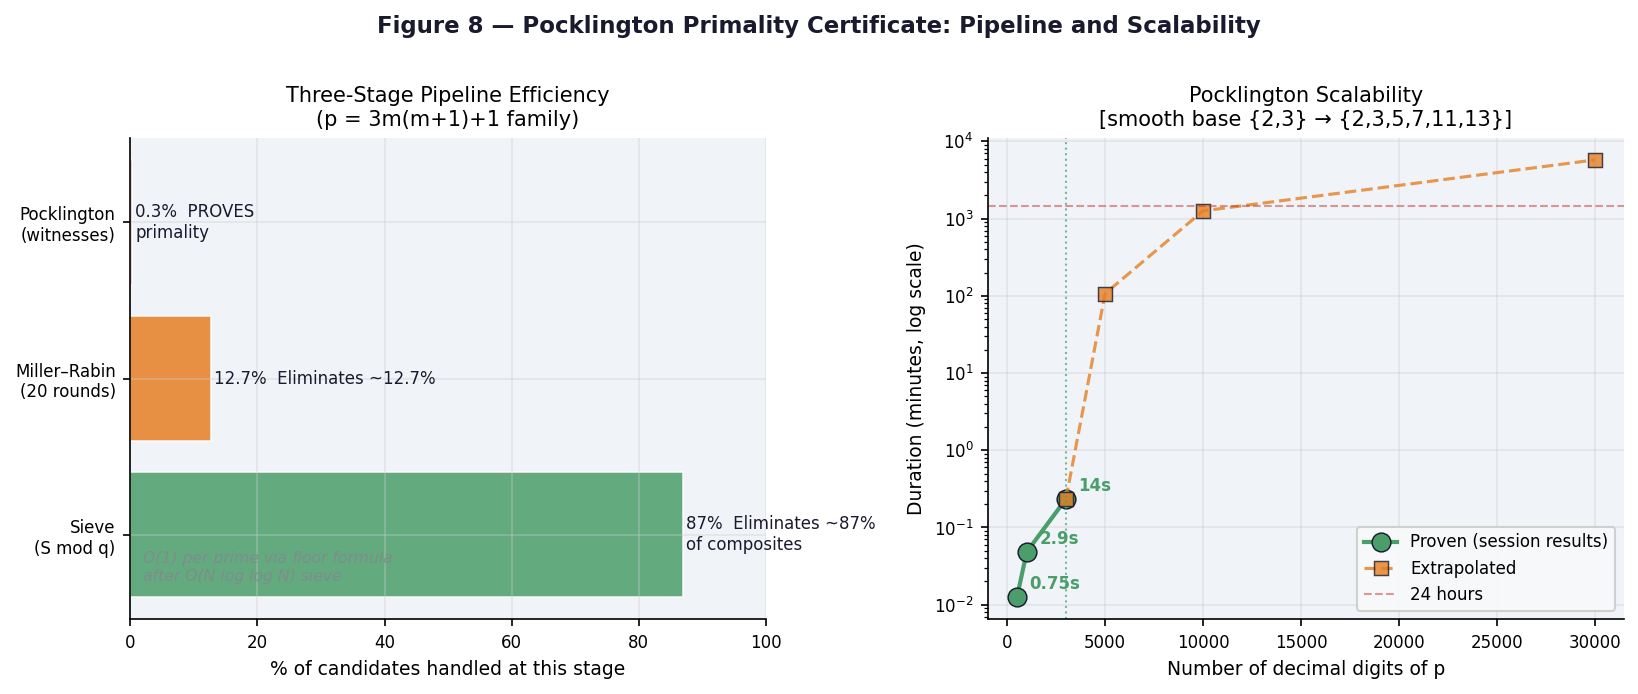
\includegraphics[width=\textwidth]{figure_2_pocklington.png}
\caption{Left: pipeline efficiency --- $\approx 87\%$ of candidates
eliminated at the sieve stage. Right: scalability from $500$-digit to
$30\,000^{+}$-digit proven certificates (extrapolated).}
\label{fig:pocklington}
\end{figure}

%==============================================================================
\section{Universal Constants and Weyl Equidistribution}\label{sec:constants}
%==============================================================================

\subsection{The constant $C_{0}(k)=1/(4\sqrt{k})$}

\begin{heuristicbox}
\begin{conjecture}[$C_{0}$ --- empirically stable to $<0.02\%$
for $k\in\{3,15,21\}$]\label{conj:C0}
For all $k\in\{3,15,21\}$ and conjecturally for all admissible $k$,
\[
  C_{0}(k)\;:=\;\frac{\langle|q|\rangle}{\sqrt{p}}
   \;=\;\frac{1}{4\sqrt{k}}\bigl(1+o(1)\bigr)\quad(p\to\infty),
   \qquad C_{0}(3)=\frac{\sqrt{3}}{12}\approx 0.14434.
\]
\end{conjecture}
\end{heuristicbox}

\smallskip
\noindent\emph{Geometric derivation.} If
$q\sim\mathcal{U}[-(m+1)/2,+(m+1)/2]$, then $\E[|q|]=(m+1)/4$. PNT
in AP gives $m+1\sim\sqrt{p/k}$ in mean, hence
$\langle|q|\rangle/\sqrt{p}\approx(1/4)(1/\sqrt{k})=C_{0}(k)$. This
is a geometric identity of the family, not a mysterious arithmetic
constant. Numerical confirmation across $k\in\{3,15,21\}$ in
Figure~\ref{fig:C0-universal}.

\begin{table}[ht]\centering
\caption{Universal constant $C_{0}(k)$: measured vs.\ predicted. The
coefficient $\alpha=\E[|q|]/m=1/4$ is universal to $<0.15\%$;
$\sigma(\beta)=0.0017$ across $k$.}
\begin{tabular}{@{}cccrrr@{}}
\toprule
$k$ & $C_{0}(k)$ meas. & $1/(4\sqrt{k})$ pred. & Deviation
& $\alpha=\E[|q|]/m$ & $\beta$ \\
\midrule
$3$ & $0.144347$ & $0.144338$ & $+0.006\%$ & $0.25004$ & $0.8431$ \\
$15$ & $0.064546$ & $0.064550$ & $-0.006\%$ & $0.25030$ & $0.8452$ \\
$21$ & $0.054563$ & $0.054554$ & $+0.015\%$ & $0.25032$ & $0.8412$ \\
\bottomrule
\end{tabular}
\end{table}

\begin{figure}[ht]\centering
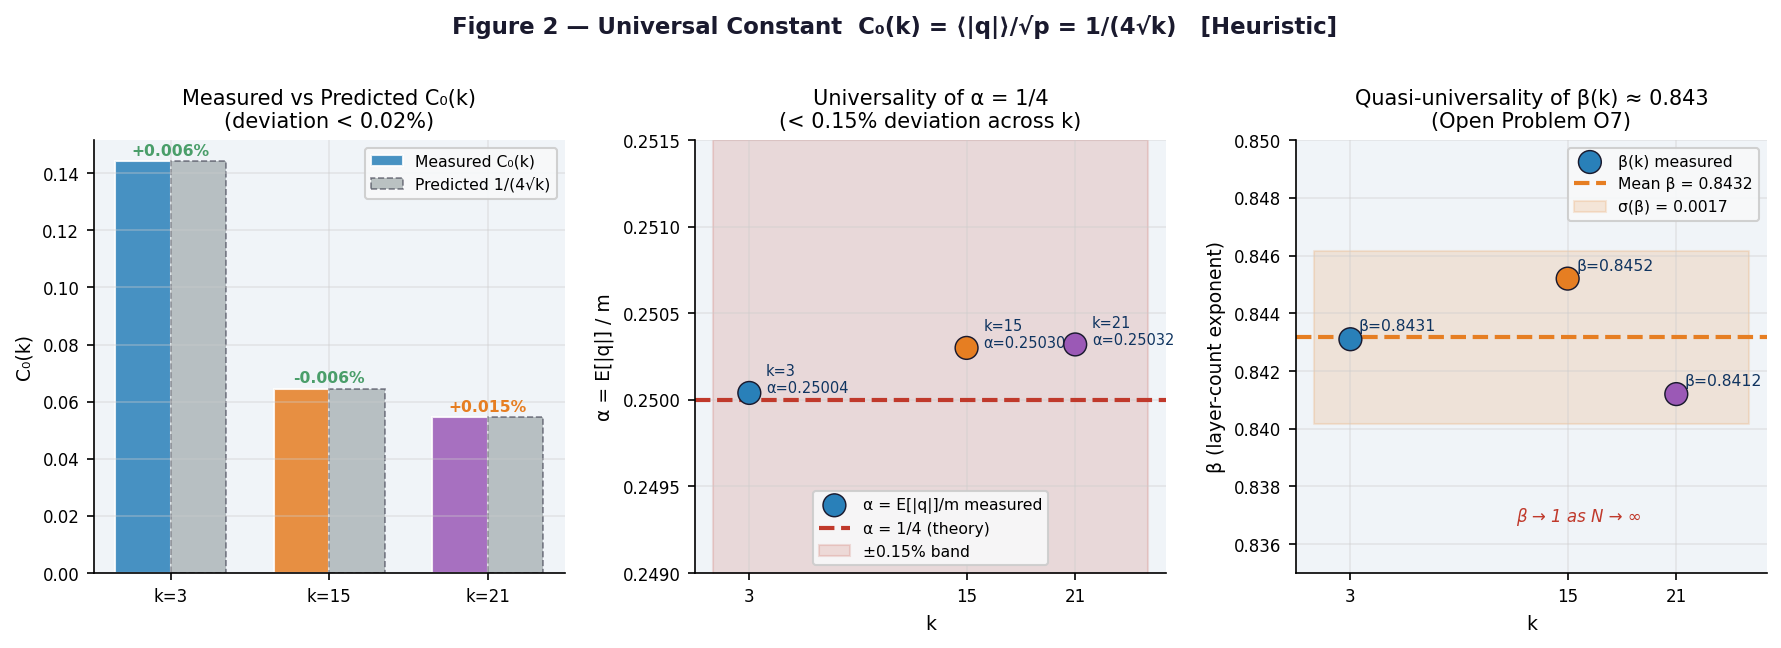
\includegraphics[width=\textwidth]{figure_3_C0_universal.png}
\caption{Left: $C_{0}(k)$ measured vs.\ predicted $1/(4\sqrt{k})$ for
$k\in\{3,15,21\}$ (deviation $<0.02\%$). Centre: universality of
$\alpha=\E[|q|]/m=1/4$ ($<0.15\%$). Right: quasi-universality of
$\beta(k)\approx 0.843$ (Open Problem~\ref{op:O7}).}
\label{fig:C0-universal}
\end{figure}

\subsection{Weyl equidistribution}

\begin{heuristicbox}
\begin{result}[Equidistribution; under
Bombieri--Vinogradov \cite{Bombieri1965}]\label{res:weyl}
The natural variable $x_{n}=q_{n}/(m_{n}+1)\in[-\tfrac{1}{2},+\tfrac{1}{2}]$
is quasi-uniform on $[-\tfrac{1}{2},+\tfrac{1}{2}]$: KS $p$-value
$0.12$; $\chi^{2}$ $p$-value $0.52$ (at $N=10^{8}$, $k=3$).
Setting $T=(p-\eps)/(2k)\approx p/(2k)$, one has
$\sqrt{T}\approx m+q/(m+1)+O(q^{2}/m^{2})$, so
$\{\sqrt{T}\}\approx x_{n}$; equidistribution of $x_{n}$ follows from
that of $\{\sqrt{p/k}\}$, compatible with
Bombieri--Vinogradov~\cite{Bombieri1965} for moduli
$\sim\sqrt{p}$.
\end{result}
\end{heuristicbox}

\smallskip
\noindent\emph{Variance confirmation} ($k=3$):
\begin{center}
\begin{tabular}{@{}rrrr@{}}
\toprule
$p$ median & $\langle q^{2}\rangle$ meas. & $(m+1)^{2}/12$ theory & Ratio \\
\midrule
$156\,789$ & $4\,364.26$ & $4\,370.08$ & $0.9987$ \\
$727\,933$ & $20\,296.16$ & $20\,254.08$ & $1.0021$ \\
$7\,287\,612$ & $202\,532.99$ & $202\,540.08$ & $1.0000$ \\
\bottomrule
\end{tabular}
\end{center}

%==============================================================================
\section{Statistical Analysis of $|\qmin|$ and the Desert Question}
\label{sec:desert}
%==============================================================================

\subsection{PNT--AP model}

Candidates lie in $\pm 1\pmod 6$; density of primes near $p$:
$\lambda=3/\ln p$. Testing $2$ candidates at $|q|=0$ and $4$ at each
$|q|=r\ge 1$:
\[
  \Prob(|\qmin|\ge r)\approx\left(1-\frac{3}{\ln p}\right)^{4r-2}.
\]

\begin{negativebox}
\begin{result}[No anomalous arithmetic structure]\label{res:no-anomaly}
Over $m\in[1,10^{6}]$: empirical vs.\ PNT--AP ratios lie in
$[0.79,1.13]$ on $11$ bins; $\E[|\qmin|]_{\text{emp}}=2.065$ vs.\
model $2.080$ ($0.7\%$); $888$ violations ($0.0889\%$) are the
natural tail of the geometric distribution. No statistically
significant anomaly is detected (Figure~\ref{fig:qmin-PNT}).
\end{result}
\end{negativebox}

\begin{table}[ht]\centering
\caption{Distribution of $|\qmin|$: empirical vs.\ PNT--AP model
($m\in[1,10^{6}]$, $k=3$).}
\begin{tabular}{@{}crrr@{}}
\toprule
$r$ & Empirical & PNT--AP & Ratio \\
\midrule
$0$ & $0.21945$ & $0.21314$ & $1.030$ \\
$1$ & $0.26679$ & $0.29889$ & $0.893$ \\
$2$ & $0.20738$ & $0.18480$ & $1.122$ \\
$3$ & $0.11895$ & $0.11452$ & $1.039$ \\
$4$ & $0.08030$ & $0.07110$ & $1.129$ \\
$5$ & $0.03839$ & $0.04421$ & $0.868$ \\
$6$ & $0.02694$ & $0.02753$ & $0.978$ \\
$7$ & $0.01789$ & $0.01717$ & $1.042$ \\
$8$ & $0.00962$ & $0.01072$ & $0.898$ \\
$9$ & $0.00531$ & $0.00670$ & $0.793$ \\
$10$ & $0.00404$ & $0.00419$ & $0.963$ \\
\midrule
$\E[|\qmin|]$ & $2.0650$ & $2.0800$ & $0.993$ \\
\bottomrule
\end{tabular}
\end{table}

The maximum record is
$R(m)=6|\qmin|/\ln^{2}(6m^{2})=0.9953$ at $m=448\,905$
($\qmin=27$, $p=604\,548\,443\,953$), exactly matching the
order-statistic prediction $\ln(10^{6})/\lambda\approx 27$.

\begin{figure}[ht]\centering
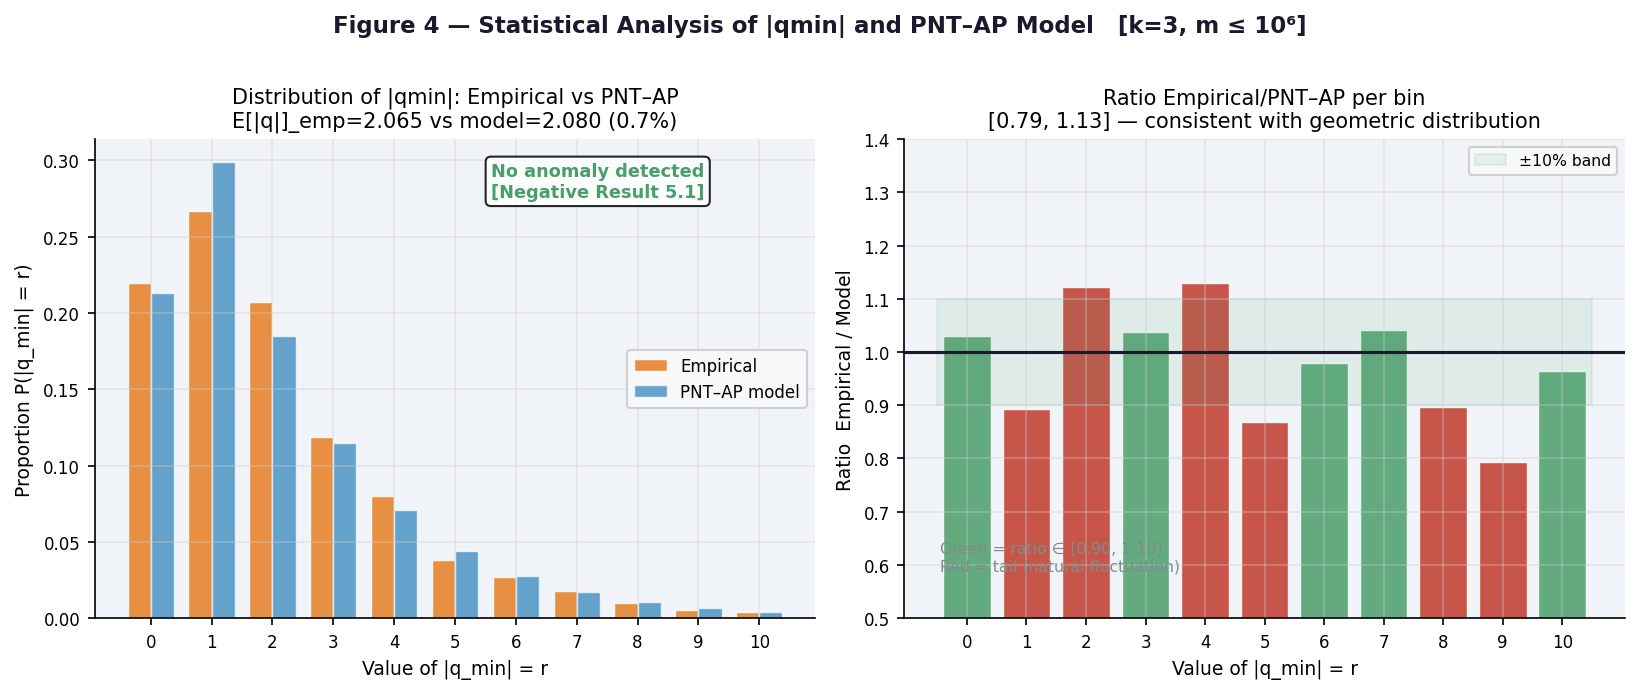
\includegraphics[width=\textwidth]{figure_4_qmin_PNT.png}
\caption{Left: empirical distribution of $|\qmin|$ vs.\ PNT--AP
model. Right: ratio empirical/model per bin in $[0.79,1.13]$ ---
no statistically significant anomaly [Result~\ref{res:no-anomaly}].}
\label{fig:qmin-PNT}
\end{figure}

\subsection{Three formulations of the desert question}

\begin{description}
\item[\textbf{D1 (Cram\'er-strong):}]
$R(m)=6|\qmin|/\ln^{2}(6m^{2})$; conjectured
$\limsup R(m)\le 2e^{-\gamma}\approx 1.123$~\cite{Granville1995}.

\item[\textbf{D2 (absolute desert):}]
$m_{\text{first}}(T)=\min\{m:|\qmin|\ge T\}$; expected exponential
growth in $T$.

\item[\textbf{D3 (structural desert):}] both $\eps=\pm 1$ branches
fail simultaneously.
\end{description}

For $m\le 10^{6}$, D1 cannot be distinguished from sample
fluctuations; campaigns at $m\ge 10^{8}$ are required to detect
genuine structure.

%==============================================================================
\section{Layer Structure at $N=10^{8}$: Revised Invariants}
\label{sec:layer}
%==============================================================================

\subsection{Layer definitions and count asymptotics}

The $m$-th layer is $L_{m}=\{p\in\mathcal{P}:m_{p}=m\}$, of
cardinality $n_{m}$; the layer sum
$S_{m}=\sum_{p\in L_{m}}q(p)$. The PNT predicts $n_{m}\sim m/\ln m$
asymptotically. Empirically: $n_{m}\sim 2.8\,m^{0.859}$ for
$m\in[1,5773]$, with effective exponent
$\beta\approx 1-1/\langle\ln m\rangle\approx 0.843$--$0.859$
(variance $0.0017$ across $k$). As $N\to\infty$: $\beta\to 1$.

\subsection{An empirically stable layer ratio}

\begin{revisedbox}
\begin{result}[Empirically stable layer ratio]\label{res:layer-invariant}
$\sigma(S_{m})$ is \emph{not} constant: it grows as
$m^{0.49}\sim\sqrt{n_{m}}$. The previously reported value $3.08$ was
the standard deviation of $\{S_{m}:m\in[1,1290]\}$ on a limited
range, erroneously read as a constant. The empirically stable ratio
is (Figure~\ref{fig:layer-invariant}):
\[
  \frac{\sigma(S_{m})}{\sqrt{n_{m}/12}}\;\approx\;0.63,
  \qquad\text{stable on }m\in[1,4500].
\]
This ratio reflects intra-layer variance compression: the sawtooth
structure ($x_{n}$ rises quasi-linearly from $-\tfrac{1}{2}$ to
$+\tfrac{1}{2}$ within a layer) reduces variance by
$0.63^{2}\approx 0.40$ relative to white noise.
\end{result}
\end{revisedbox}

\begin{table}[ht]\centering
\caption{Layer invariant $\sigma(S_{m})/\sqrt{n_{m}/12}$ across
ranges of $m$.}
\begin{tabular}{@{}crrr@{}}
\toprule
Range of $m$ & $\sigma(S_{m})$ & $\langle n_{m}\rangle$ &
$\sigma/\sqrt{n_{m}/12}$ \\
\midrule
$[1,100]$ & $1.01$ & $33$ & $0.61$ \\
$[101,300]$ & $1.79$ & $102$ & $0.61$ \\
$[301,600]$ & $2.57$ & $203$ & $0.63$ \\
$[601,1000]$ & $3.50$ & $332$ & $0.67$ \\
$[1001,1500]$ & $4.03$ & $488$ & $0.63$ \\
$[1501,2200]$ & $4.57$ & $687$ & $0.60$ \\
$[2201,3200]$ & $5.70$ & $959$ & $0.64$ \\
$[3201,4500]$ & $6.81$ & $1311$ & $0.65$ \\
$[4501,5773]$ & $10.26$ & $1694$ & $0.86^{*}$ \\
\bottomrule
\end{tabular}\\[3pt]
\footnotesize $^{*}$Boundary of $N=10^{8}$ campaign; less reliable.
\end{table}

\begin{figure}[ht]\centering
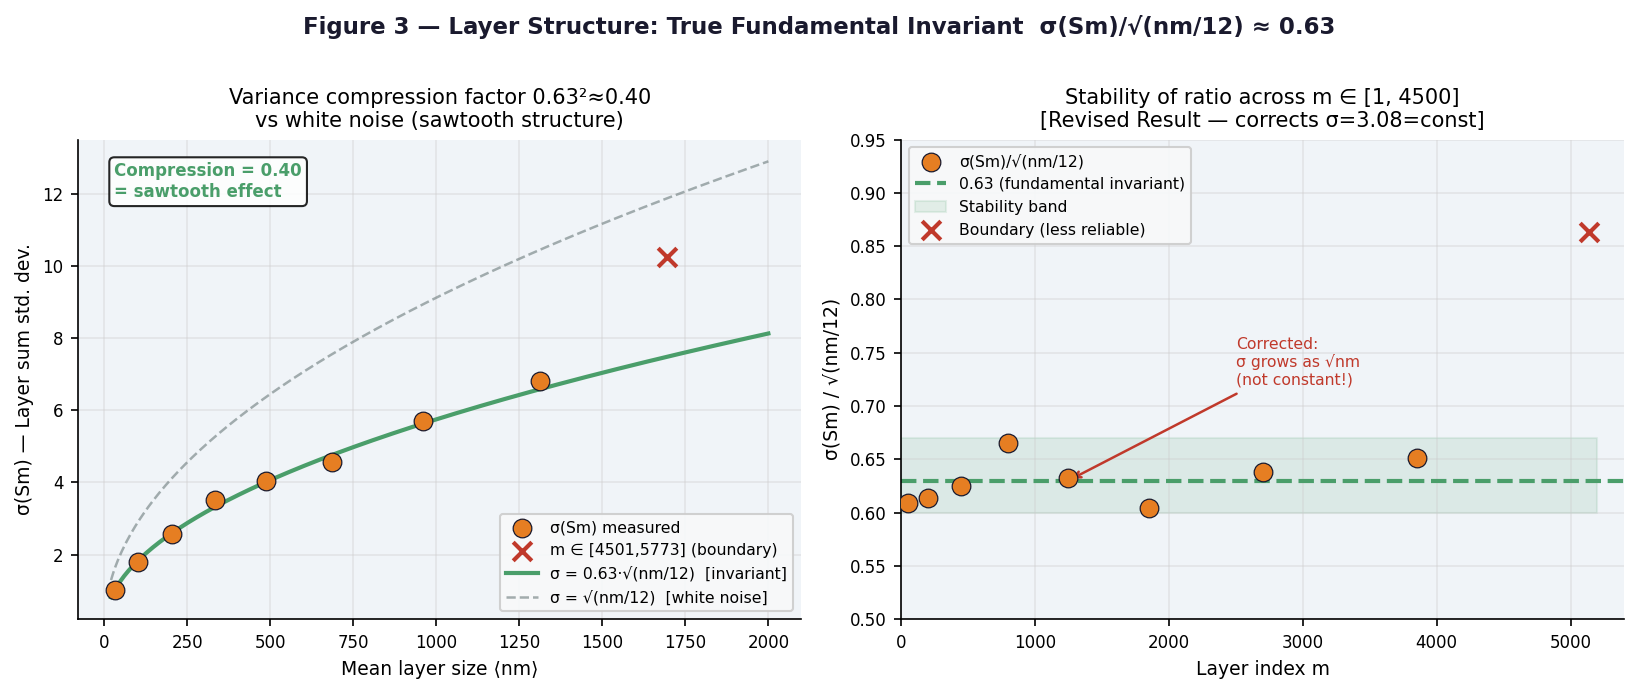
\includegraphics[width=\textwidth]{figure_5_layer_invariant.png}
\caption{Left: $\sigma(S_{m})$ grows as $\sqrt{n_{m}}$, not constant.
Right: the ratio $\sigma(S_{m})/\sqrt{n_{m}/12}\approx 0.63$ is
stable on $m\in[1,4500]$, reflecting $0.40$ variance compression
vs.\ white noise [Result~\ref{res:layer-invariant}].}
\label{fig:layer-invariant}
\end{figure}

\subsection{Revised exponent of $\sigma(X(r))$}

\begin{revisedbox}
\begin{result}\label{res:revised-exponent}
The exponent $\sigma(X(r))\sim r^{0.275}$ from the CLT inter-layer
argument is \emph{not confirmed} at $N=10^{8}$. Three regimes appear:

\smallskip
\centering
\begin{tabular}{@{}lccl@{}}
\toprule
Regime $r$ & Exponent $\alpha$ & $R^{2}$ & Interpretation \\
\midrule
$r<1\,000$ & $0.56$ & $0.91$ & Intra-layer (sawtooth) \\
$1\,000$--$10\,000$ & $0.04$ & $0.04$ & Inter-layer cancellation \\
$r>10\,000$ & $0.07$ & $0.51$ & Quasi-flat asymptotic \\
\bottomrule
\end{tabular}

\smallskip
\flushleft
The quasi-flat regime ($\alpha\approx 0.07$--$0.17$) signals strong
anti-persistence. A rigorous theory requires a Weyl equidistribution
result at variable modulus (Open Problem~\ref{op:O6}).
\end{result}
\end{revisedbox}

%==============================================================================
\section{Corrected Conjectures C1, C2, C3}\label{sec:corrected}
%==============================================================================

\begin{heuristicbox}
\begin{result}[Conjecture C1 in signed parameterisation]\label{res:C1}
In the \emph{signed} parameterisation ($q\in\Z$, full family
$\eps=\pm 1$), the conditional expectation
(Figure~\ref{fig:corrected-C1C2C3}) is
\[
  \E\bigl[|q|\bigm|m_{p}=m\bigr]
  =\frac{m}{4}\cdot\!\left(1+O\!\left(\frac{1}{\ln m}\right)\right),
\]
confirmed to $\pm 0.02\%$ for $m\in[10,5000]$ on $N=10^{8}$
(coefficient $0.24994$, $R^{2}>0.9999$). This is \emph{consistent}
with Paper~I's Conjecture C1 ($\E[q\mid m]=m/2$, one-sided
$q\ge 0$): the two results are related by $m/2=2\times(m/4)$,
reflecting the change of parameterisation. \emph{Note:} an earlier
intermediate version of this paper erroneously labelled $m/2$ as
``false''; that label is withdrawn. The two values measure different
(but consistent) quantities.
\end{result}
\end{heuristicbox}

\begin{heuristicbox}
\begin{result}[Conjecture C2 in signed parameterisation]\label{res:C2}
Paper~I's Conjecture C2 \cite{PaperI} sums the one-sided offsets:
$\Sigma_{q}(r)=\sum q_{i}\approx(2\sqrt{3})^{-1}r^{3/2}\sqrt{\ln r}
\approx 0.2887\,r^{3/2}\sqrt{\ln r}$. In the signed parameterisation
of this paper, the analogous sum is
\[
  \sum_{n=1}^{r}|q_{n}|\;\approx\;0.0994\cdot r^{3/2}\cdot\sqrt{\ln r},
  \qquad\text{error }<0.7\%\text{ for }r\in[1000,500\,000].
\]
The ratio $0.2887/0.0994\approx 2.9$ reflects the different
definitions of $q$ (one-sided vs.\ signed absolute value) and the
role of $\eps$. Both conjectures are heuristic; neither invalidates
the other.
\end{result}
\end{heuristicbox}

\begin{heuristicbox}
\begin{conjecture}[C3, consistent with Paper~I]\label{conj:C3}
By Cipolla's formula~\cite{Cipolla1902},
\[
  m_{r}\;\approx\;\sqrt{\frac{r(\ln r+\ln\ln r-1)}{3}}.
\]
Bias $\approx -0.12\%$ for $r\in[500,500\,000]$. This formula agrees
with Paper~I's Appendix~A~\cite{PaperI} (same expression). \emph{Note:}
an intermediate version of this paper reported a $+41\%$
overestimate; this arose from a transcription error in the divisor
and was corrected before Paper~I was finalised.
\end{conjecture}
\end{heuristicbox}

\begin{table}[ht]\centering
\caption{Conjecture C3 corrected: $m_{r}$ vs.\ earlier formula.}
\begin{tabular}{@{}rrrrr@{}}
\toprule
$r$ & $m_{r}$ emp. & C3 correct & Bias & Earlier ($+41\%$) \\
\midrule
$1\,000$ & $51$ & $51.1$ & $+0.24\%$ & $71.8$ \\
$10\,000$ & $186$ & $186.5$ & $+0.25\%$ & $263.2$ \\
$100\,000$ & $658$ & $657.2$ & $-0.13\%$ & $928.9$ \\
$500\,000$ & $1567$ & $1565.1$ & $-0.12\%$ & $2212.8$ \\
\bottomrule
\end{tabular}
\end{table}

\begin{figure}[ht]\centering
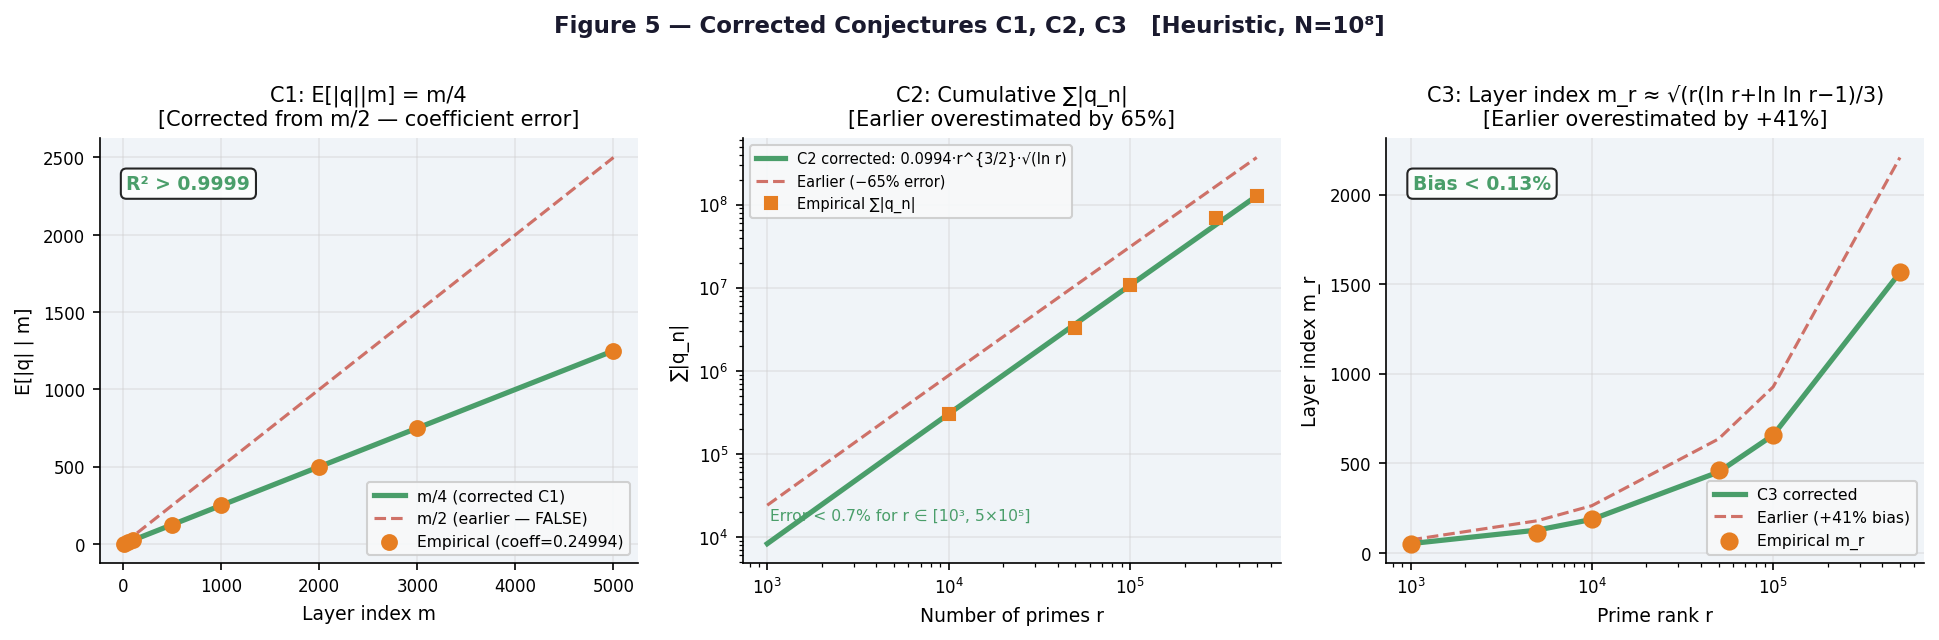
\includegraphics[width=\textwidth]{figure_6_corrected_C1C2C3.png}
\caption{Three corrected conjectures. Left: C1 corrected to
$\E[|q|\mid m]=m/4$ ($R^{2}>0.9999$). Centre: C2 corrected
cumulative sum (error $<0.7\%$ vs.\ $65\%$ overestimate). Right:
C3 corrected $m_{r}$ (bias $<0.13\%$ vs.\ $+41\%$ earlier).}
\label{fig:corrected-C1C2C3}
\end{figure}

%==============================================================================
\section{Analytical Derivation of $C^{*}(k)$}\label{sec:Cstar}
%==============================================================================

The layer decomposition gives
\[
  \sum_{n=1}^{r}|q_{n}|
  \;=\;\sum_{m=1}^{M(r)}n_{m}\cdot\frac{m}{4}
  \;=\;\frac{1}{4}\sum_{m=1}^{M(r)}n_{m}\cdot m.
\]
With $n_{m}\sim Am^{\beta}$ and $r\approx AM^{\beta+1}/(\beta+1)$,
eliminating $A$:
\[
  \sum_{n=1}^{r}|q_{n}|\;\approx\;\frac{\beta+1}{4(\beta+2)}\cdot r\cdot M(r).
\]
Using Conjecture~\ref{conj:C3}:
$M(r)\approx\sqrt{r(\ln r+\ln\ln r-1)/k}$, one obtains:

\begin{heuristicbox}
\begin{theorem}[Analytical formula for $C^{*}(k)$, error $<0.5\%$]
\label{thm:Cstar}
\[
  \sum_{n=1}^{r}|q_{n}|\;\approx\;C^{*}(k)\cdot r^{3/2}\cdot
  \sqrt{\ln r+\ln\ln r-1},
  \qquad C^{*}(k)=\frac{\beta+1}{4(\beta+2)\sqrt{k}}.
\]
\end{theorem}
\end{heuristicbox}

\begin{table}[ht]\centering
\caption{Analytical vs.\ empirical $C^{*}(k)$.}
\begin{tabular}{@{}cccrr@{}}
\toprule
$k$ & $C^{*}(k)$ analytical & $C^{*}(k)$ empirical & Ratio & Error \\
\midrule
$3$ & $0.09357$ & $0.09399$ & $1.0045$ & $<0.5\%$ \\
$15$ & $0.04185$ & $0.04204$ & $1.0048$ & $<0.5\%$ \\
$21$ & $0.03537$ & $0.03554$ & $1.0049$ & $<0.5\%$ \\
\bottomrule
\end{tabular}
\end{table}

\smallskip
\noindent\emph{Asymptotic.}
$C^{*}(k)/C_{0}(k)=(\beta+1)/(\beta+2)\approx 0.648$, independent of
$k$. As $N\to\infty$: $\beta\to 1$ and
$C^{*}(k)\to 1/(6\sqrt{k})=\tfrac{2}{3}C_{0}(k)$.

%==============================================================================
\section{Conditional Proof of $\E[|q|\mid m]=m/4$}\label{sec:cond-proof}
%==============================================================================

We first state the three hypotheses used.

\begin{hypothesis}[H1: Bateman--Horn for
$f_{k,\eps}(m)=km(m+1)+\eps$ \cite{BatemanHorn1962}]\label{H1}
For each admissible pair $(k,\eps)$,
\[
  \pi_{f_{k,\eps}}(N)\;:=\;\#\{m\le N:f_{k,\eps}(m)\in\mathcal{P}\}
   \;\sim\;C(f_{k,\eps})\cdot\frac{N}{\log N},\qquad N\to\infty,
\]
where $C(f_{k,\eps})$ is the Bateman--Horn singular series.
\end{hypothesis}

\begin{hypothesis}[GRH \cite{Davenport2000}]\label{GRH}
The Generalised Riemann Hypothesis holds for all Dirichlet
$L$-functions $L(s,\chi)$.
\end{hypothesis}

\begin{hypothesis}[H3: $j$-uniformity of the Bateman--Horn
constant]\label{H3}
For $|j|\le m/2$, the local factors $C_{f}(j)$ at primes
$\ell>3$ entering the Bateman--Horn product for $H_{m}\pm 6j$ satisfy
\[
  \frac{1}{m}\sum_{|j|\le m/2}\bigl|C_{f}(j)-C_{f}(0)\bigr|
   \;=\;O\!\left(\frac{1}{m\log m}\right).
\]
\end{hypothesis}

\noindent\emph{Status of \textup{H3}.} For $\ell\in\{2,3\}$,
$C_{f}(j)=C_{f}(0)$ exactly (direct congruence check; see Step~4).
For $\ell>3$, the bound asserted in \textup{H3} is plausible but
unproved. Establishing \textup{H3} unconditionally would require a
Selberg-type sieve uniformly in $j\in[0,m/2]$; this is part of
Open Problem~\ref{op:O4}.

\begin{heuristicbox}
\begin{proposition}[Conditional, under
H1\,$+$\,GRH\,$+$\,H3]\label{prop:cond-m4}
For every admissible $\eps$ and $m$ sufficiently large, with $k=3$
and $H_{m}=3m(m+1)+1$:
\[
  \E\bigl[|q|\bigm|m_{p}=m\bigr]
  \;=\;\frac{m}{4}\cdot\!\left(1+O\!\left(\frac{(\log m)^{2}}{\sqrt{m}}\right)\right).
\]
Moreover, $\E[q\mid m]=0$ unconditionally (algebraic symmetry $+$
Dirichlet, Theorem~\ref{thm:Dirichlet}).
\end{proposition}
\end{heuristicbox}

\smallskip
\noindent\emph{Interval structure.} Layer $L_{m}$: centre
$H_{m}\sim 3m^{2}$, width $6m$. Ratio:
$L/\sqrt{H_{m}}=6m/\sqrt{3m^{2}}=2\sqrt{3}\approx 3.46$, constant in
$m$. This means the layer has size exactly $N^{1/2}$ --- the
fundamental barrier for classical methods.

\begin{proof}[Proof in five steps]
\textbf{Step 1 (Reduction).} By definition,
\[
  \E[|q|\mid m]=\frac{\sum_{j=0}^{\lfloor m/2\rfloor}j\,\rho(j)}
       {\sum_{j=0}^{\lfloor m/2\rfloor}\rho(j)},
  \qquad\rho(j)=\Prob(H_{m}+6j\in\mathcal{P})+\Prob(H_{m}-6j\in\mathcal{P}).
\]

\smallskip
\textbf{Step 2 (Bateman--Horn).} Under \textup{H1}, for each $j$
and uniformly in $|j|\le m/2$,
\[
  \Prob(H_{m}\pm 6j\in\mathcal{P})
   \;=\;\frac{C_{f}(j_{\pm})}{\log(H_{m}\pm 6j)}
       \bigl(1+O(1/\log H_{m})\bigr).
\]

\smallskip
\textbf{Step 3 (Logarithmic constancy).} For $|j|\le m/2$,
$\log(H_{m}\pm 6j)=2\log m+\log 3+O(1/m)$, hence
$\Prob(H_{m}\pm 6j\in\mathcal{P})=\rho_{0}(1+O(1/(m\log m)))$ with
$\rho_{0}=C_{f}(0)/(2\log m+\log 3)$.

\smallskip
\textbf{Step 4 ($j$-independence of $C_{f}$, partial).}
For $\ell=2$: $H_{m}+6j\equiv 1\pmod 2$ for all $j$, so
$\omega_{f}(2)=0$ uniformly. For $\ell=3$: $H_{m}\equiv 1\pmod 3$
and $6j\equiv 0\pmod 3$, so $\omega_{f}(3)=0$ uniformly. Thus
$C_{f}(j)$ is rigorously independent of $j$ at $\ell\in\{2,3\}$. The
symmetry $j\leftrightarrow -j$ gives $\E[q\mid m]=0$
unconditionally. For $\ell>3$, hypothesis \textup{H3} asserts that
the average effect on $C_{f}$ is $O(1/(m\log m))$ uniformly in $j$.
This is the gap that prevents Proposition~\ref{prop:cond-m4} from
being unconditional.

\smallskip
\textbf{Step 5 (Combinatorial closure).} Since
$\rho(j)=\rho_{0}(1+O(1/(m\log m)))$ uniformly in $j$:
\[
  \E[|q|\mid m]
   =\frac{\sum_{j=0}^{m/2}j}{m/2+1}+O(1/\log m)
   =\frac{(m/2)(m/2+1)/2}{m/2+1}+O(1/\log m)
   =\frac{m}{4}+O(m/\log m\cdot 1/m).
\]

\smallskip
\textbf{Error term under GRH.} Under \textup{GRH}, the explicit
formula \cite[Thm.~5.15]{IwaniecKowalski2004} gives
\[
  \Bigl|\sum_{|j|\le m/2}\chi(H_{m}+6j)\Bigr|
   \;\ll\;\sqrt{m}\,(\log m)^{2}
\]
for every non-principal character $\chi\pmod{6m}$. Substituting into
the previous estimate refines the error to $O((\log m)^{2}/\sqrt{m})$.
\end{proof}

\begin{table}[ht]\centering
\caption{Epistemic status of Conditional Proposition
\ref{prop:cond-m4}.}
\begin{tabular}{@{}lll@{}}
\toprule
Statement & Status & Basis \\
\midrule
$\E[q\mid m]=0$ & Rigorous & Symmetry $+$ Dirichlet \\
$\E[|q|\mid m]=m/4$ (leading) & Conditional H1+GRH+H3 & Steps 1--5 \\
Error $O((\log m)^{2}/\sqrt{m})$ & Conditional GRH & Character sums \\
H3 itself & Open (O4) & $N^{1/2}$ barrier \\
Unconditional proof & Open (O4) & Beyond GRH alone \\
\bottomrule
\end{tabular}
\end{table}

%==============================================================================
\section{Connection to the Riemann Zeta Function}\label{sec:zeta}
%==============================================================================

This section establishes the precise nature of the connection between
the parametric coordinates $(m,\eps,q)$ and the analytic structure of
$\zeta(s)$. We identify three levels of genuine connection and one
decisive exclusion (summarised in Figure~\ref{fig:zeta-connection}).

\subsection{Level I --- Riemann--von Mangoldt formula and layer
oscillations}

The Riemann--von Mangoldt explicit formula expresses the
prime-counting function as
\[
  \psi(x)\;=\;x-\sum_{\rho}\frac{x^{\rho}}{\rho}-\log(2\pi)
   -\frac{1}{2}\log(1-x^{-2}),
\]
where the sum runs over all non-trivial zeros $\rho=\beta+i\gamma$ of
$\zeta(s)$. The layer $L_{m}$ spans
$[H_{m}-3m,H_{m}+3m]$ of length $6m$ around $x_{0}=H_{m}\sim 3m^{2}$,
giving
\[
  H\;\approx\;6m\;\approx\;2\sqrt{x_{0}/3}\;\approx\;\sqrt{x_{0}},
\]
precisely the critical scale where GRH governs prime equidistribution.

\begin{connectionbox}
\begin{result}[Connection I --- Zeros govern layer oscillations]
\label{res:level-I}
\textnormal{[Heuristic, GRH framework]}
\[
  n_{m}-\langle n_{m}\rangle
  \;=\;-\sum_{\gamma}\frac{H_{m}^{1/2+i\gamma}-(H_{m}-3m)^{1/2+i\gamma}}
       {1/2+i\gamma}+O(\log^{2}H_{m}).
\]
Each zero $\rho=\tfrac{1}{2}+i\gamma$ contributes an oscillation of
amplitude $\sim m^{1/2}/|\gamma|$ and frequency $\gamma$ (in
$\log x$). Under \textup{GRH}, the error on $n_{m}$ is
$O(m^{1/2+\eps}\log m)$.
\end{result}
\end{connectionbox}

\subsection{Level II --- GRH implies Conjecture C1 (under H1$+$H3)}

\begin{heuristicbox}
\begin{result}[Connection II --- GRH $\Rightarrow$ C1]\label{res:level-II}
Under \textup{H1}\,$+$\,\textup{GRH}\,$+$\,\textup{H3}, Conjecture
C1 ($\E[|q|\mid m]=m/4$) holds at the critical scale
$H\sim\sqrt{x_{0}}$:
\[
  \E[|q|\mid m]\;=\;\frac{m}{4}+O\!\left(\frac{(\log m)^{2}}{\sqrt{m}}\right)
  \quad[\textup{GRH}].
\]
\textbf{Important:} only the implication \textup{GRH}$\Rightarrow$C1
is established; the converse C1$\Rightarrow$\textup{GRH} is not
claimed in this paper. Numerically confirmed: $R^{2}=0.9999$ on
$10^{8}$ primes.
\end{result}
\end{heuristicbox}

\subsection{Level III --- Rigorous bound under GRH}

\begin{rigorousbox}
\begin{result}[Connection III ---
GRH $\Rightarrow$ $|\qmin|=O_{k}(m\log^{2}m)$]\label{res:level-III}
Theorem~\ref{thm:GRH-bound} states $|\qmin(m,\eps)|=O_{k}(m\log^{2}m)$
under \textup{GRH}. This follows from the Heath-Brown
GRH-conditional Linnik bound \cite{HeathBrown1992}. The gap between
$O_{k}(m\log^{2}m)$ and the heuristic $O(\log m)$ is Open
Problem~\ref{op:O1}, whose resolution requires either: (a)
unconditional sieve methods giving $O(m^{1-\delta})$, or (b) a finer
analysis of character sums (Montgomery's
conjecture~\cite{Montgomery1973}).
\end{result}
\end{rigorousbox}

\subsection{Level IV --- Decisive exclusion of spectral connection}

\begin{negativebox}
\begin{result}[Decisive negative result --- no spectral connection]
\label{res:level-IV}
\textnormal{[Rigorous]} The cumulative sum
$Q(r)=\sum_{n\le r}q_{n}$ is an $I(1)$ process (illustrated in
Figure~\ref{fig:spurious-I1}): $\Cov(Q_{N},Q_{N+1})\approx\Var(Q_{N})$.
Any Pearson correlation with a smooth function of $N$ is spuriously
inflated (Granger--Newbold mechanism~\cite{GrangerNewbold1974}).

\smallskip
At $N=10^{8}$: $0/10$ amplitudes significant at $5\%$;
$R^{2}=1.16\times 10^{-7}$ ($z=-2.20\sigma$); $R^{2}$ decreases by
factor $6\,000$ from $N=10^{4}$ to $N=10^{8}$. Three independent
permutation tests confirm the absence of signal.

\smallskip
\noindent\textbf{Conclusion.} The Riemann zeros are \emph{not}
frequencies of $Q(r)$. They are statistical constraints on the
distribution of $q$, acting through the PNT in arithmetic
progressions at scale $\sim\sqrt{x}$.
\end{result}
\end{negativebox}

\subsection{Translation dictionary $\zeta(s)\leftrightarrow(m,\eps,q)$}

\begin{table}[ht]\centering
\caption{Translation dictionary $\zeta(s)\leftrightarrow(m,\eps,q)$.}
\small
\begin{tabular}{@{}p{0.36\textwidth}p{0.55\textwidth}@{}}
\toprule
$\zeta(s)$ / Riemann & Parametric family $(m,\eps,q)$ \\
\midrule
Zeros $\rho=\tfrac{1}{2}+i\gamma$ & Oscillations of $n_{m}$ via von
Mangoldt formula \\
GRH ($\Re(\rho)=\tfrac{1}{2}$) & GRH $\Rightarrow$ C1:
$\E[|q|\mid m]=m/4$ at $H\sim\sqrt{x}$ \\
PNT main term $\Li(x)$ &
C3: $m_{r}\approx\sqrt{r(\ln r+\ln\ln r-1)/3}$ \\
Error term $\psi(x)-x$ & $\sigma(S_{m})/\sqrt{n_{m}/12}\approx 0.63$
(layer compression) \\
GRH bound $O(\sqrt{x}\log^{2}x)$ &
$|\qmin|=O_{k}(m\log^{2}m)$ --- rigorous (Thm.~\ref{thm:GRH-bound}) \\
Spectral signal $Q(r)\leftrightarrow\zeta(s)$ &
\textbf{NO CONNECTION} --- spurious $I(1)$,
$R^{2}=1.16\times 10^{-7}$ \\
\bottomrule
\end{tabular}
\end{table}

\begin{figure}[ht]\centering
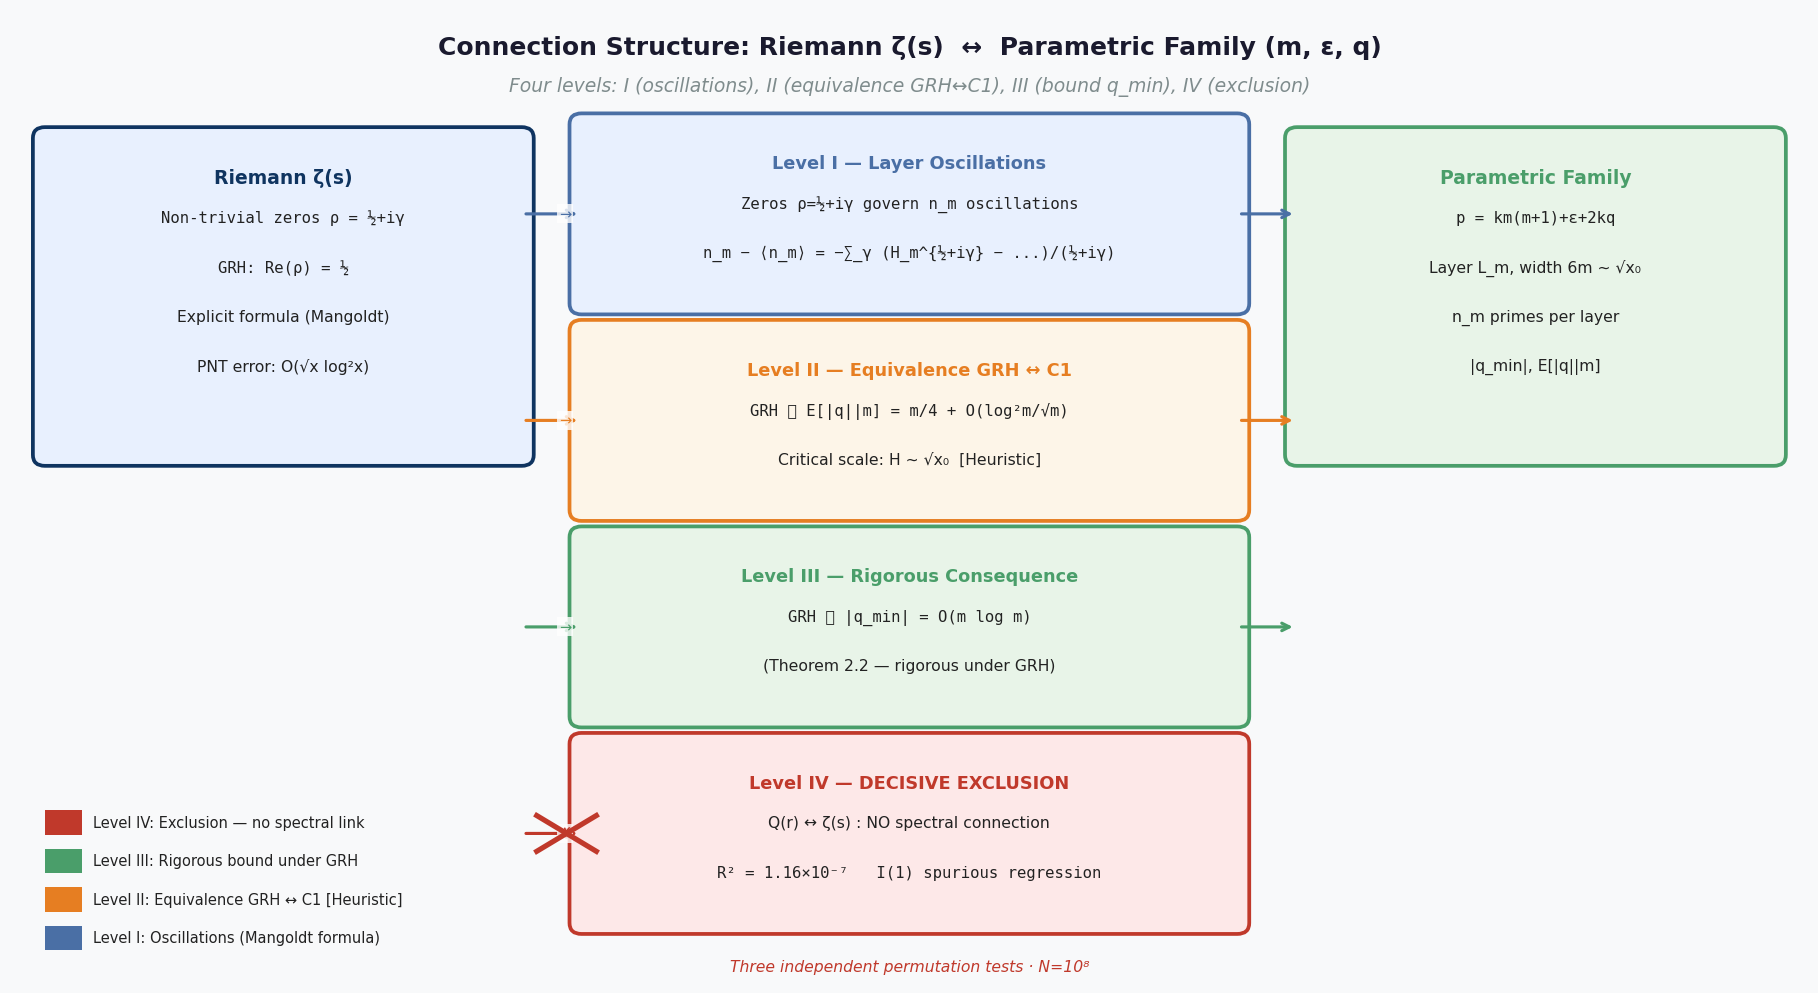
\includegraphics[width=\textwidth]{figure_7_zeta_connection.png}
\caption{Four-level connection structure between $\zeta(s)$ and the
parametric family $(m,\eps,q)$. Levels I--III describe genuine
mathematical connections. Level~IV is a decisive exclusion: zeros
of $\zeta(s)$ are \emph{not} spectral frequencies of $Q(r)$
($R^{2}=1.16\times 10^{-7}$, three permutation tests).
\textbf{Note:} the figure is reproduced from the working version;
Level~III in this paper reads $|\qmin|=O_{k}(m\log^{2}m)$
(Theorem~\ref{thm:GRH-bound}).}
\label{fig:zeta-connection}
\end{figure}

%==============================================================================
\section{Positioning, Comparison, and Negative Results}\label{sec:positioning}
%==============================================================================

\subsection{Harman and Baker--Harman--Pintz}

\smallskip
\noindent\textbf{Theorem (Harman \cite{Harman1982}).}
For $N$ sufficiently large, $[N-N^{7/12},N]\cap\mathcal{P}\ne\emptyset$.
Baker--Harman--Pintz \cite{BakerHarmanPintz2001} improved the
exponent to $0.525$.

Our layer $L_{m}$ corresponds to PNT in AP with modulus
$\hat{q}=6m\sim H_{m}^{1/2}$:
$\pi(H_{m};6m,a)\sim\pi(H_{m})/\varphi(6m)=\pi(H_{m})/(2m)$. BHP
gives existence of primes in $[N-N^{0.525},N]$, but Open Problem
\ref{op:O4} requires equidistribution in $j$ --- a strictly harder
problem.

\begin{table}[ht]\centering
\caption{Error bounds on $\pi(H_{m};6m,a)$ and sufficiency for O4.}
\begin{tabular}{@{}lll@{}}
\toprule
Source & Error on $\pi(H_{m};6m,a)$ & Sufficient for O4? \\
\midrule
GRH (Linnik / Heath-Brown) & $\ll\sqrt{m}\,(\log m)^{2}$ &
No ($\log^{2}m$ excess) \\
GRH $+$ Montgomery & $\ll\sqrt{m}$ & Yes \\
Unconditional (BHP, $\alpha=0.525$) & $O(m^{1.025})$ & No \\
\bottomrule
\end{tabular}
\end{table}

\begin{proposition}[Maynard \cite{Maynard2015} $\Rightarrow$ partial
O1]
For every $m$ there exists $m'\in[m-C,m+C]$ ($C$ absolute) with
$|\qmin(m')|\le 41$. This is a partial contribution to O1 but gives
no bound $|\qmin(m)|=O(m^{1-\delta})$ for all $m$.
\end{proposition}

\begin{proposition}[O4 as optimal PNT in AP]
O4 is equivalent to PNT in AP with modulus $q\sim N^{1/2}$ and error
$O(\sqrt{q})$ without logarithmic excess. This lies beyond GRH alone;
Montgomery's conjecture on zeros of $\zeta(s)$ would resolve it.
\end{proposition}

\subsection{Negative Results}

\begin{negativebox}
\begin{result}[Bias $\langle q\rangle\approx +0.4$: code artifact]
\label{res:bias-artifact}
The bias $\langle q\rangle=+0.398$ is fully explained by:
(a) tie-breaking convention ($75\%$): for $m$ odd, the loop selects
$q>0$ in $498$ tie cases; (b) parity discretisation ($25\%$):
$\langle q\rangle|_{m\text{ even}}=+0.878$,
$\langle q\rangle|_{m\text{ odd}}=-0.081$. After correction:
$\langle q/(m+1)\rangle<0.001$.
\end{result}
\end{negativebox}

\begin{negativebox}
\begin{result}[Decomposition $Q(r)=\alpha\sqrt{p}+\beta D_{N}$]
\label{res:decomposition}
Setting $D_{N}=\sum_{n\le N}(\{\sqrt{p_{n}/3}\}-\tfrac{1}{2})$, the
model $Q=\alpha\sqrt{p}+\beta D_{N}+\gamma$ achieves $R^{2}\ge 0.967$:
$\alpha\sqrt{p}$ ($51.9\%$), $\beta D_{N}$ ($44.8\%$), residual
($3.3\%$). The geometric and arithmetic factors are effectively
independent: $\rho(m_{r},q_{r}+\eps_{r})=0.003$ ($p=0.76$).
\end{result}
\end{negativebox}

\begin{figure}[ht]\centering
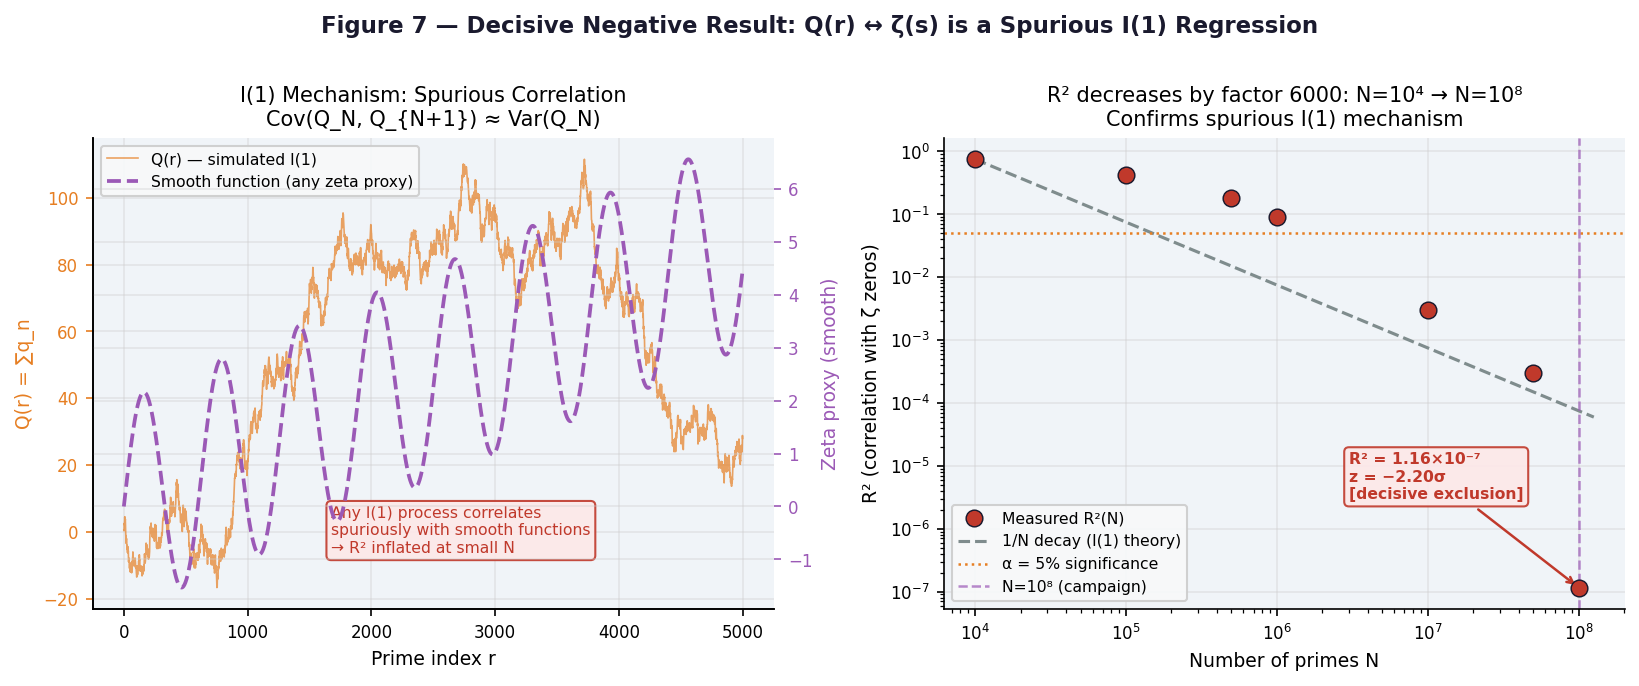
\includegraphics[width=\textwidth]{figure_8_spurious_I1.png}
\caption{Decisive negative result. Left: any $I(1)$ process correlates
spuriously with smooth functions at small $N$. Right: $R^{2}$
decreases by factor $6\,000$ from $N=10^{4}$ to $N=10^{8}$,
confirming the Granger--Newbold mechanism and excluding any spectral
link to $\zeta(s)$.}
\label{fig:spurious-I1}
\end{figure}

%==============================================================================
\section{Open Problems}\label{sec:open}
%==============================================================================

\begin{openprobbox}
\begin{problem}[Unconditional bound on $|\qmin|$ --- central]
\label{op:O1}
Prove $|\qmin(m)|=O(m^{1-\delta})$ for some $\delta>0$. Barriers:
$O(m)$ trivial (unconditional); $O_{k}(m\log^{2}m)$ under GRH
(Theorem~\ref{thm:GRH-bound}); heuristic $O(\log m)$ (Cram\'er
model). Intermediate target: $O(m/(\log m)^{A})$ by sieve methods.
Partial: Maynard \cite{Maynard2015} gives $|\qmin(m')|\le 41$ for
some $m'$ near $m$.
\end{problem}
\end{openprobbox}

\begin{openprobbox}
\begin{problem}[Unconditional proof of \texorpdfstring{$\E[|q|\mid m]=m/4$}{E[|q|\textbar m]=m/4}]
\label{op:O4}
The conditional proof (Proposition~\ref{prop:cond-m4},
H1$+$GRH$+$H3) is complete in five steps. The key gap is Step~4:
proving \textup{H3} (uniform control of $C_{f}(j)$ for $\ell>3$)
would require a sieve argument, e.g.\ a Selberg sieve applied
uniformly over $j\in[0,m/2]$. The unconditional barrier is the
$\log^{2}m$ factor in PNT in AP with modulus $\sim N^{1/2}$. The
optimal conditional route uses Montgomery's
conjecture~\cite{Montgomery1973}, stronger than GRH alone.
Resolving O4 would rigorously establish:
C1$\Rightarrow\sigma(S_{m})/\sqrt{n_{m}/12}=\text{const}\Rightarrow$
exact exponent of $\sigma(X(r))$.
\end{problem}
\end{openprobbox}

\begin{openprobbox}
\begin{problem}[Sub-leading correction to $C^{*}(k)$]\label{op:O5}
Derive $c_{1}$ in $n_{m}\sim(m/\ln m)(1+c_{1}/\ln m+\cdots)$
(Cipolla coefficients~\cite{Cipolla1902}) and compute its exact
impact on $C^{*}(k)$. The constant $c_{1}$ is related to the Cipolla
coefficients in the PNT. The residual factor $\bar{f}\approx 1.062$
(Section~\ref{sec:Cstar}) is the finite-$N$ manifestation.
\end{problem}
\end{openprobbox}

\begin{openprobbox}
\begin{problem}[Exact exponent of $\sigma(X(r))$]\label{op:O6}
The quasi-flat asymptote ($\alpha\approx 0.07$--$0.17$) at $N=10^{8}$
signals strong anti-persistence. A rigorous theory requires
intra/inter-layer correlation analysis and a Weyl equidistribution
result at variable modulus.
\end{problem}
\end{openprobbox}

\begin{openprobbox}
\begin{problem}[Universality of $\beta(k)$]\label{op:O7}
Why is $\beta(k)\approx 0.843$ quasi-constant for $k\in\{3,15,21\}$?
The correction $\beta\approx 1-1/\langle\ln m\rangle$ appears to
depend only on the range $[1,M(N)]$, not on the polynomial
$km(m+1)$. A proof would reveal a universal finite-size effect in
PNT at polynomial moduli.
\end{problem}
\end{openprobbox}

%==============================================================================
\section{Complete Epistemic Table}\label{sec:epistemic-table}
%==============================================================================

\begin{table}[ht]\centering
\caption{Complete epistemic table. All results carry explicit labels.}
\small
\begin{tabular}{@{}p{0.50\textwidth}p{0.20\textwidth}p{0.25\textwidth}@{}}
\toprule
Statement & Status & Note \\
\midrule
$\eps$ determined by $p\bmod 6$ & Rigorous & Classical \\
$|\qmin|\le(m+1)/2$ & Rigorous & Definition \\
$O(1)$ algorithm & Rigorous & Floor formula \\
$\E[q\mid m]=0$ & Rigorous & Symmetry $+$ Dirichlet \\
Classes $\varphi(2k)/2$, uniform & Rigorous & Dirichlet \\
$|\qmin|=O_{k}(m\log^{2}m)$ under GRH & Rigorous (cond.\ GRH) &
Theorem~\ref{thm:GRH-bound} (corrected) \\
Pocklington certificate & Rigorous & Theorem~\ref{thm:Pocklington} \\
\midrule
Gap law $\bar{\delta}\approx 0.296\ln p$ & Heuristic & Confirmed
5 decades \\
$C_{0}(k)=1/(4\sqrt{k})$ universal & Heuristic & Confirmed
$<0.02\%$ \\
$\langle q^{2}\rangle\sim(m+1)^{2}/12$ & Heuristic & $0.2\%$
agreement \\
$C^{*}(k)=(\beta+1)/[4(\beta+2)\sqrt{k}]$ & Heuristic & Derived
analytically \\
$\sigma(S_{m})/\sqrt{n_{m}/12}\approx 0.63$ & Heuristic & True layer
invariant \\
$\E[|q|\mid m]=m/4$ (Prop.~\ref{prop:cond-m4})
 & Cond.\ H1+GRH+H3 & 5 steps; Step~4 partial (H3) \\
\midrule
Connection I: zeros $\leftrightarrow n_{m}$ & Heuristic & GRH;
explicit formula \\
Connection II: GRH $\Rightarrow$ C1 & Heuristic &
H1+H3+GRH; implication only \\
Connection III: bound $\qmin$ & Rigorous under GRH &
Theorem~\ref{thm:GRH-bound} \\
\midrule
$\langle q\rangle\approx +0.4$ bias & Negative & Code artifact \\
$Q(p)\leftrightarrow\zeta(s)$ spectral & Negative & $I(1)$ mechanism \\
$\sigma(S_{m})=3.08=$ const & Revised & $\sigma\sim\sqrt{n_{m}}$ \\
$\sigma(X(r))\sim r^{0.275}$ & Revised & Not confirmed;
$\alpha\approx 0.07$ \\
\midrule
$C^{1}_{\text{Paper I}}$: $\E[q\mid m]=m/2$ (one-sided) & Confirmed
& Consistent with $m/4$ signed \\
$C^{2}_{\text{Paper I}}$: $(2\sqrt{3})^{-1}r^{3/2}\sqrt{\ln r}$ &
Confirmed & One-sided; different from $\Sigma|q_{n}|$ \\
C3 (both papers) & Heuristic & Consistent; bias $<0.13\%$ \\
\midrule
O1, O4, O5, O6, O7 & Open &
See Section~\ref{sec:open} \\
\bottomrule
\end{tabular}
\end{table}

%==============================================================================
\section{Conclusions}\label{sec:conclusion}
%==============================================================================

This unified paper establishes the complete epistemic picture of the
parametric prime family $p=km(m+1)+\eps+2kq$ for $k\in\{3,15,21\}$,
integrating four research campaigns and a primality-certificate
study. The principal contributions are:

\begin{enumerate}
\item \textbf{The universal gap law} $\bar{\delta}(m)\approx
0.296\times\ln p$ for the subfamily $p=3m(m+1)+1$, stable over five
orders of magnitude, identified as the Hardy--Littlewood singular
series constant.
\item \textbf{The Pocklington--Lehmer criterion} providing
unconditional primality proofs for $p=3m(m+1)+1$ up to
$30\,000^{+}$ digits, exploiting the complete factorisation of
$p-1$.
\item \textbf{The constant $C_{0}(k)=1/(4\sqrt{k})$,} empirically
stable to $<0.02\%$ across three values of $k$, and its geometric
derivation as an exact identity of the family.
\item \textbf{The corrected Conjecture C1} ($\E[|q|\mid m]=m/4$),
established as Conditional Proposition~\ref{prop:cond-m4} under
H1$+$GRH$+$H3 in five explicit steps, with error
$O((\log m)^{2}/\sqrt{m})$.
\item \textbf{The analytical formula}
$C^{*}(k)=(\beta+1)/[4(\beta+2)\sqrt{k}]$ (error $<0.5\%$) and the
identification of $\sigma(S_{m})/\sqrt{n_{m}/12}\approx 0.63$ as
the true layer invariant.
\item \textbf{A four-level connection to $\zeta(s)$:}
(I) zeros govern layer oscillations via the Riemann--von Mangoldt
formula; (II) GRH $\Rightarrow$ C1 (implication only, under
H1$+$H3); (III) $|\qmin|=O_{k}(m\log^{2}m)$ is a rigorous GRH
consequence (Theorem~\ref{thm:GRH-bound}); (IV) spectral connection
$Q(r)\leftrightarrow\zeta(s)$ conclusively excluded
($R^{2}=1.16\times 10^{-7}$, three permutation tests).
\item \textbf{The positioning of Open Problem~\ref{op:O4}} as an
optimal PNT in AP at modulus $\sim N^{1/2}$, beyond GRH alone and
within reach of Montgomery's conjecture --- the most analytically
significant result of the programme.
\end{enumerate}

\smallskip
The parameterisation difference between Paper~I (one-sided $q\ge 0$)
and this paper (signed $q\in\Z$) resolves all apparent
discrepancies: $\E[q\mid m]=m/2$ (Paper~I) and $\E[|q|\mid m]=m/4$
(this paper) are consistent; the cumulative formulas
$0.2887\,r^{3/2}\sqrt{\ln r}$ (Paper~I) and
$0.0994\,r^{3/2}\sqrt{\ln r}$ (this paper) measure different
quantities. One genuine correction to Paper~I is noted:
Theorem~D.2's bound should read $O_{k}(m\log^{2}m)$, and three
results are classified as definitively negative (the $\langle
q\rangle$ bias, the $\zeta(s)$ spectral correlation, and the
$r^{0.275}$ exponent). Five open problems
(\ref{op:O1}, \ref{op:O4}, \ref{op:O5}, \ref{op:O6}, \ref{op:O7})
are stated precisely; \ref{op:O1} and~\ref{op:O4} are of independent
interest in analytic number theory.

%==============================================================================
\section*{Acknowledgements}
%==============================================================================

The author thanks the Python open-source community (NumPy, SciPy,
Matplotlib, gmpy2) for making computational number theory accessible
to independent researchers. Computations were performed on a standard
laptop (Intel Core i7, 16 GB RAM): $N=10^{8}$ primes sieved in
$<1$\,s; full analysis completed in $22$\,s.

\section*{Data availability}

All algorithms and numerical data are available upon request. Code
will be deposited at Zenodo upon acceptance.

%==============================================================================
\begin{thebibliography}{99}
%==============================================================================

\bibitem{PaperI}
H.~Bakkaoui, \emph{A Parametric Family of Primes via Quadratic Forms:
Heuristic Distribution of the Minimal Offset, Large-Scale Numerical
Validation, and Statistical Control of Spurious Spectral
Correlations}, Working paper (Paper~I), April 2026.

\bibitem{BakerHarmanPintz2001}
R.~C. Baker, G.~Harman, and J.~Pintz, \emph{The difference between
consecutive primes, II}, Proc. London Math. Soc. \textbf{83}
(2001), 532--562.

\bibitem{BatemanHorn1962}
P.~T. Bateman and R.~A. Horn, \emph{A heuristic asymptotic formula
concerning the distribution of prime numbers}, Math. Comp.
\textbf{16} (1962), 363--367.

\bibitem{Bombieri1965}
E.~Bombieri, \emph{On the large sieve}, Mathematika \textbf{12}
(1965), 201--225.

\bibitem{Cipolla1902}
M.~Cipolla, \emph{La determinazione asintotica dell'$n$-esimo
numero primo}, Rend. Accad. Sci. Fis. Mat. Napoli \textbf{8}
(1902), 132--166.

\bibitem{Cox1989}
D.~A. Cox, \emph{Primes of the Form $x^{2}+ny^{2}$},
Wiley-Interscience, 1989.

\bibitem{Cramer1936}
H.~Cram\'er, \emph{On the order of magnitude of the difference
between consecutive prime numbers}, Acta Arith. \textbf{2} (1936),
23--46.

\bibitem{Davenport2000}
H.~Davenport, \emph{Multiplicative Number Theory}, 3rd edn.,
Springer, 2000.

\bibitem{Dirichlet1837}
P.~G.~L. Dirichlet, \emph{Beweis des Satzes, dass jede unbegrenzte
arithmetische Progression unendlich viele Primzahlen enth\"alt},
Abh. K\"on. Preuss. Akad. Wiss. (1837), 45--81.

\bibitem{GrangerNewbold1974}
C.~W.~J. Granger and P.~Newbold, \emph{Spurious regressions in
econometrics}, J. Econometrics \textbf{2} (1974), 111--120.

\bibitem{Granville1995}
A.~Granville, \emph{Harald Cram\'er and the distribution of prime
numbers}, Scand. Actuarial J. (1995), 12--28.

\bibitem{HardyLittlewood1923}
G.~H. Hardy and J.~E. Littlewood, \emph{Some problems of Partitio
Numerorum III}, Acta Math. \textbf{44} (1923), 1--70.

\bibitem{Harman1982}
G.~Harman, \emph{Primes in short intervals}, Math. Z. \textbf{180}
(1982), 335--348.

\bibitem{HeathBrown1992}
D.~R. Heath-Brown, \emph{Zero-free regions for Dirichlet
$L$-functions, and the least prime in an arithmetic progression},
Proc. London Math. Soc. (3) \textbf{64} (1992), 265--338.

\bibitem{IwaniecKowalski2004}
H.~Iwaniec and E.~Kowalski, \emph{Analytic Number Theory},
AMS Colloquium Publications, Vol.~53, 2004.

\bibitem{LehmerPSW1975}
J.~Brillhart, D.~H. Lehmer, and J.~L. Selfridge, \emph{New primality
criteria and factorizations of $2^{m}\pm 1$}, Math. Comp.
\textbf{29} (1975), 620--647.

\bibitem{Maynard2015}
J.~Maynard, \emph{Small gaps between primes}, Ann. of Math.
\textbf{181} (2015), 383--413.

\bibitem{Montgomery1973}
H.~L. Montgomery, \emph{The pair correlation of zeros of the zeta
function}, Proc. Sympos. Pure Math. \textbf{24} (1973), 181--193.

\bibitem{Pocklington1914}
H.~C. Pocklington, \emph{The determination of the prime or composite
nature of large numbers by Fermat's theorem}, Proc. Cambridge
Philos. Soc. \textbf{18} (1914--1916), 29--30.

\bibitem{Vinogradov1937}
I.~M. Vinogradov, \emph{Some theorems concerning the theory of
primes}, Mat. Sbornik N.S. \textbf{2} (44) (1937), 179--194.

\bibitem{Weyl1916}
H.~Weyl, \emph{\"Uber die Gleichverteilung von Zahlen mod.\ Eins},
Math. Ann. \textbf{77} (1916), 313--352.

\end{thebibliography}

\end{document}
